%-----------------------------------------------------------------------------------------
% Autor dieser Vorlage:
% Stefan Macke (http://fachinformatiker-anwendungsentwicklung.net)
% Permalink zur Vorlage: http://fiae.link/LaTeXVorlageFIAE
% Lizenz: Creative Commons 4.0 Namensnennung - Weitergabe unter gleichen Bedingungen
% -----------------------------------------------------------------------------------------

\documentclass[
	ngerman,
	toc=listof, % Abbildungsverzeichnis sowie Tabellenverzeichnis in das Inhaltsverzeichnis aufnehmen
	toc=bibliography, % Literaturverzeichnis in das Inhaltsverzeichnis aufnehmen
	footnotes=multiple, % Trennen von direkt aufeinander folgenden Fußnoten
	parskip=half, % vertikalen Abstand zwischen Absätzen verwenden anstatt horizontale Einrückung von Folgeabsätzen
	numbers=noendperiod, % Den letzten Punkt nach einer Nummerierung entfernen (nach DIN 5008)
	12pt
]{scrartcl}
\pdfminorversion=5 % erlaubt das Einfügen von pdf-Dateien bis Version 1.7, ohne eine Fehlermeldung zu werfen (keine Garantie für fehlerfreies Einbetten!)
\usepackage[utf8]{inputenc} % muss als erstes eingebunden werden, da Meta/Packages ggfs. Sonderzeichen enthalten

% !TEX root = Ausarbeitung.tex

% Hinweis: der Titel muss zum Inhalt des Projekts passen und den zentralen Inhalt des Projekts deutlich herausstellen
\newcommand{\titel}{Projektplan für das Projekt}
\newcommand{\untertitel}{Projektplanung}
\newcommand{\kompletterTitel}{\titel{} -- \untertitel}


\newcommand{\betriebLogo}{logo.png}


\newcommand{\betreff}{Schriftliche Ausarbeitung im Modul Projektplanung}
 % Metadaten zu diesem Dokument (Autor usw.)
% !TEX root = ../Ausarbeitung.tex

% Anpassung an Landessprache ---------------------------------------------------
\usepackage{babel}
\usepackage{lipsum}
% Umlaute ----------------------------------------------------------------------
%   Umlaute/Sonderzeichen wie äüöß direkt im Quelltext verwenden (CodePage).
%   Erlaubt automatische Trennung von Worten mit Umlauten.
% ------------------------------------------------------------------------------
\usepackage[T1]{fontenc}
\usepackage{textcomp} % Euro-Zeichen etc.
% Schrift ----------------------------------------------------------------------
%\usepackage{lmodern} % bessere Fonts
\usepackage{relsize} % Schriftgröße relativ festlegen

% Tabellen ---------------------------------------------------------------------
\PassOptionsToPackage{table}{xcolor}
\usepackage{tabularx}
% für lange Tabellen
\usepackage{longtable}
\usepackage{array}
\usepackage{ragged2e}
\usepackage{lscape}
\newcolumntype{w}[1]{>{\raggedleft\hspace{0pt}}p{#1}} % Spaltendefinition rechtsbündig mit definierter Breite

% Grafiken ---------------------------------------------------------------------
\usepackage[dvips,final]{graphicx} % Einbinden von JPG-Grafiken ermöglichen
\usepackage{graphics} % keepaspectratio
\usepackage{float} % zum Umfließen von Bildern
\usepackage{wrapfig} % zum Umfließen von Bildern
\graphicspath{{Bilder/}} % hier liegen die Bilder des Dokuments




% Sonstiges --------------------------------------------------------------------
\usepackage[titles]{tocloft} % Inhaltsverzeichnis DIN 5008 gerecht einrücken
\usepackage{amsmath,amsfonts} % Befehle aus AMSTeX für mathematische Symbole
\usepackage{enumitem} % anpassbare Enumerates/Itemizes
\usepackage{xspace} % sorgt dafür, dass Leerzeichen hinter parameterlosen Makros nicht als Makroendezeichen interpretiert werden

\usepackage{makeidx} % für Index-Ausgabe mit \printindex
\usepackage[printonlyused]{acronym} % es werden nur benutzte Definitionen aufgelistet

\usepackage{datetime} % Angabe des Build-Datums auf dem Deckblatt

\usepackage{url}  %url im Literaturverteichnis brechen
\def\UrlBreaks{\do\/\do-}

% Einfache Definition der Zeilenabstände und Seitenränder etc.
\usepackage{setspace}
\usepackage{geometry}

% Symbolverzeichnis
\usepackage[intoc]{nomencl}
\let\abbrev\nomenclature
\renewcommand{\nomname}{Abkürzungsverzeichnis}
\setlength{\nomlabelwidth}{.25\hsize}
\renewcommand{\nomlabel}[1]{#1 \dotfill}
\setlength{\nomitemsep}{-\parsep}

\usepackage{varioref} % Elegantere Verweise. „auf der nächsten Seite“
\usepackage{url} % URL verlinken, lange URLs umbrechen etc.

\usepackage{chngcntr} % fortlaufendes Durchnummerieren der Fußnoten
% \usepackage[perpage]{footmisc} % Alternative: Nummerierung der Fußnoten auf jeder Seite neu

\usepackage{ifthen} % bei der Definition eigener Befehle benötigt
\usepackage{todonotes} % definiert u.a. die Befehle \todo und \listoftodos
\usepackage[square]{natbib} % wichtig für korrekte Zitierweise
\usepackage{float}
% PDF-Optionen -----------------------------------------------------------------
\usepackage{pdfpages}
\pdfminorversion=5 % erlaubt das Einfügen von pdf-Dateien bis Version 1.7, ohne eine Fehlermeldung zu werfen (keine Garantie für fehlerfreies Einbetten!)
\usepackage[
    bookmarks,
    bookmarksnumbered,
    bookmarksopen=true,
    bookmarksopenlevel=1,
    colorlinks=true,
% diese Farbdefinitionen zeichnen Links im PDF farblich aus
    linkcolor=AOBlau, % einfache interne Verknüpfungen
    anchorcolor=AOBlau,% Ankertext
    citecolor=AOBlau, % Verweise auf Literaturverzeichniseinträge im Text
    filecolor=AOBlau, % Verknüpfungen, die lokale Dateien öffnen
    menucolor=AOBlau, % Acrobat-Menüpunkte
    urlcolor=AOBlau,
% diese Farbdefinitionen sollten für den Druck verwendet werden (alles schwarz)
    %linkcolor=black, % einfache interne Verknüpfungen
    %anchorcolor=black, % Ankertext
    %citecolor=black, % Verweise auf Literaturverzeichniseinträge im Text
    %filecolor=black, % Verknüpfungen, die lokale Dateien öffnen
    %menucolor=black, % Acrobat-Menüpunkte
    %urlcolor=black,
%
    %backref, % Quellen werden zurück auf ihre Zitate verlinkt
    pdftex,
    plainpages=false, % zur korrekten Erstellung der Bookmarks
    pdfpagelabels=true, % zur korrekten Erstellung der Bookmarks
    hypertexnames=false, % zur korrekten Erstellung der Bookmarks
    linktocpage % Seitenzahlen anstatt Text im Inhaltsverzeichnis verlinken
]{hyperref}
% Befehle, die Umlaute ausgeben, führen zu Fehlern, wenn sie hyperref als Optionen übergeben werden
\hypersetup{
    pdftitle={\titel -- \untertitel},
    pdfsubject={\titel -- \untertitel},
    pdfkeywords={\titel -- \untertitel},
}


% zum Einbinden von Programmcode -----------------------------------------------
\usepackage{listings}
\usepackage{xcolor}
\definecolor{hellgelb}{rgb}{1,1,0.9}
\definecolor{colKeys}{rgb}{0,0,1}
\definecolor{colIdentifier}{rgb}{0,0,0}
\definecolor{colComments}{rgb}{0,0.5,0}
\definecolor{colString}{rgb}{1,0,0}

\definecolor{lstwhite}{HTML}{000000}
\definecolor{lstblue}{HTML}{0000ff}
\definecolor{lstgreen}{HTML}{a31515}
\definecolor{lstbg}{HTML}{ffffff}

\lstset{
    float=hbp,
	basicstyle=\color{lstwhite},%\ttfamily\footnotesize,
    identifierstyle=\color{lstwhite},
    keywordstyle=\color{lstblue},
    stringstyle=\color{lstgreen},
    commentstyle=\color{lstwhite},
    backgroundcolor=\color{lstbg},
    columns=flexible,
    tabsize=2,
    frame=single,
    extendedchars=true,
    showspaces=false,
    showstringspaces=false,
    numbers=left,
    numberstyle=\footnotesize,
    breaklines=true,
    breakautoindent=true,
	captionpos=b,
    framesep=5pt,
    xleftmargin=0pt,
    xrightmargin=0pt,
}
\lstdefinelanguage{cs}{
    language=[Sharp]C,
    frame=lrb
	sensitive=false,
	morecomment=[l]{//},
	morecomment=[s]{/*}{*/},
	morestring=[b]",
	morekeywords={
		abstract,event,new,struct,as,explicit,null,switch
		base,extern,object,this,bool,false,operator,throw,
		break,finally,out,true,byte,fixed,override,try,
		case,float,params,typeof,catch,for,private,uint,
		char,foreach,protected,ulong,checked,goto,public,unchecked,
		class,if,readonly,unsafe,const,implicit,ref,ushort,
		continue,in,return,using,decimal,int,sbyte,virtual,
		default,interface,sealed,volatile,delegate,internal,short,void,
		do,is,sizeof,while,double,lock,stackalloc,
		else,long,static,enum,namespace,string},
}
\lstdefinelanguage{natural}{
	sensitive=false,
	morecomment=[l]{/*},
	morestring=[b]",
	morestring=[b]',
	alsodigit={-,*},
	morekeywords={
		DEFINE,DATA,LOCAL,END-DEFINE,WRITE,CALLNAT,PARAMETER,USING,
		IF,NOT,END-IF,ON,*ERROR-NR,ERROR,END-ERROR,ESCAPE,ROUTINE,
		PERFORM,SUBROUTINE,END-SUBROUTINE,CONST,END-FOR,END,FOR,RESIZE,
		ARRAY,TO,BY,VALUE,RESET,COMPRESS,INTO,EQ},
}
\lstdefinelanguage{php}{
	sensitive=false,
	morecomment=[l]{/*},
	morestring=[b]",
	morestring=[b]',
	alsodigit={-,*},
	morekeywords={
		abstract,and,array,as,break,case,catch,cfunction,class,clone,const,
		continue,declare,default,do,else,elseif,enddeclare,endfor,endforeach,
		endif,endswitch,endwhile,extends,final,for,foreach,function,global,
		goto,if,implements,interface,instanceof,namespace,new,old_function,or,
		private,protected,public,static,switch,throw,try,use,var,while,xor
		die,echo,empty,exit,eval,include,include_once,isset,list,require,
		require_once,return,print,unset},
}


\lstdefinelanguage{docker}{
    keywords={FROM, RUN, COPY, ADD, ENTRYPOINT, CMD,  ENV, ARG, WORKDIR, EXPOSE, LABEL, USER, VOLUME, STOPSIGNAL, ONBUILD, MAINTAINER},
    keywordstyle=\color{lstblue}\bfseries,
    identifierstyle=\color{lstwhite},
    sensitive=false,
    comment=[l]{\#},
    commentstyle=\color{purple}\ttfamily,
    stringstyle=\color{lstgreen}\ttfamily,
    morestring=[b]',
    morestring=[b]"
}

\lstdefinelanguage{docker-compose}{
    keywords={image, environment, ports, container_name, ports, volumes, links},
    keywordstyle=\color{blue}\bfseries,
    identifierstyle=\color{black},
    sensitive=false,
    comment=[l]{\#},
    commentstyle=\color{purple}\ttfamily,
    stringstyle=\color{red}\ttfamily,
    morestring=[b]',
    morestring=[b]"
}
\lstdefinelanguage{docker-compose-2}{
    keywords={version, volumes, services},
    keywordstyle=\color{blue}\bfseries,
    keywords=[2]{image, environment, ports, container_name, ports, links, build},
    keywordstyle=[2]\color{olive}\bfseries,
    identifierstyle=\color{black},
    sensitive=false,
    comment=[l]{\#},
    commentstyle=\color{purple}\ttfamily,
    stringstyle=\color{red}\ttfamily,
    morestring=[b]',
    morestring=[b]"
}

\lstset{basicstyle=\ttfamily,
    showstringspaces=false,
    commentstyle=\color{red},
    keywordstyle=\color{blue},
    inputencoding=utf8,
    extendedchars=true
} % verwendete Packages
% !TEX root = ../Ausarbeitung.tex

% Seitenränder -----------------------------------------------------------------
\setlength{\topskip}{\ht\strutbox} % behebt Warnung von geometry
\geometry{a4paper,left=30mm,right=30mm,top=30mm,bottom=35mm}

\usepackage[
	automark, % Kapitelangaben in Kopfzeile automatisch erstellen
	headsepline, % Trennlinie unter Kopfzeile
	ilines % Trennlinie linksbündig ausrichten
]{scrpage2}

% Kopf- und Fußzeilen ----------------------------------------------------------
\pagestyle{scrheadings}
% chapterpagestyle gibt es nicht in scrartcl
%\renewcommand{\chapterpagestyle}{scrheadings}
\clearscrheadfoot

% Kopfzeile
\renewcommand{\headfont}{\normalfont} % Schriftform der Kopfzeile
\ihead{\textsc{\titel}\\[0.5ex] \textit{\headmark}}
\chead{}
\ohead{\includegraphics[scale=0.1]{\betriebLogo}}
\setlength{\headheight}{15mm} % Höhe der Kopfzeile
%\setheadwidth[0pt]{textwithmarginpar} % Kopfzeile über den Text hinaus verbreitern (falls Logo den Text überdeckt)

% Fußzeile
\ifoot{\today}
\cfoot{}
\ofoot{\pagemark}

% Überschriften nach DIN 5008 in einer Fluchtlinie
% ------------------------------------------------------------------------------

% Abstand zwischen Nummerierung und Überschrift definieren
% > Schön wäre hier die dynamische Berechnung des Abstandes in Abhängigkeit
% > der Verschachtelungstiefe des Inhaltsverzeichnisses
\newcommand{\headingSpace}{1.5cm}

% Abschnittsüberschriften im selben Stil wie beim Inhaltsverzeichnis einrücken
\renewcommand*{\othersectionlevelsformat}[3]{
  \makebox[\headingSpace][l]{#3\autodot}
}

% Für die Einrückung wird das Paket tocloft benötigt
%\cftsetindents{chapter}{0.0cm}{\headingSpace}
\cftsetindents{section}{0.0cm}{\headingSpace}
\cftsetindents{subsection}{0.0cm}{\headingSpace}
\cftsetindents{subsubsection}{0.0cm}{\headingSpace}
\cftsetindents{figure}{0.0cm}{\headingSpace}
\cftsetindents{table}{0.0cm}{\headingSpace}


% Allgemeines
% ------------------------------------------------------------------------------

\onehalfspacing % Zeilenabstand 1,5 Zeilen
\frenchspacing % erzeugt ein wenig mehr Platz hinter einem Punkt

% Schusterjungen und Hurenkinder vermeiden
\clubpenalty = 10000
\widowpenalty = 10000
\displaywidowpenalty = 10000

% Quellcode-Ausgabe formatieren
%\lstset{numbers=left, numberstyle=\tiny, numbersep=5pt, breaklines=true}
\lstset{emph={square}, emphstyle=\color{red}, emph={[2]root,base}, emphstyle={[2]\color{blue}}}

\counterwithout{footnote}{section} % Fußnoten fortlaufend durchnummerieren
\setcounter{tocdepth}{\subsubsectionlevel} % im Inhaltsverzeichnis werden die Kapitel bis zum Level der subsubsection übernommen
\setcounter{secnumdepth}{\subsubsectionlevel} % Kapitel bis zum Level der subsubsection werden nummeriert

% Aufzählungen anpassen
\renewcommand{\labelenumi}{\arabic{enumi}.}
\renewcommand{\labelenumii}{\arabic{enumi}.\arabic{enumii}.}
\renewcommand{\labelenumiii}{\arabic{enumi}.\arabic{enumii}.\arabic{enumiii}}

% Tabellenfärbung:
\definecolor{heading}{rgb}{0.64,0.78,0.86}
\definecolor{odd}{rgb}{0.9,0.9,0.9}

% Schriftart
\usepackage[sfdefault, scale=1, light]{roboto}  % Roboto als Schrifart
\usepackage[T1]{fontenc}
\usepackage{newtxsf}
 % Definitionen zum Aussehen der Seiten
% !TEX root = ../Ausarbeitung.tex

% Abkürzungen, ggfs. mit korrektem Leerraum
\newcommand{\bs}{$\backslash$\xspace}
\newcommand{\bspw}{bspw.\xspace}
\newcommand{\bzw}{bzw.\xspace}
\newcommand{\ca}{ca.\xspace}
\newcommand{\dahe}{\mbox{d.\,h.}\xspace}
\newcommand{\etc}{etc.\xspace}
\newcommand{\eur}[1]{\mbox{#1\,\texteuro}\xspace}
\newcommand{\evtl}{evtl.\xspace}
\newcommand{\ggfs}{ggfs.\xspace}
\newcommand{\Ggfs}{Ggfs.\xspace}
\newcommand{\gqq}[1]{\glqq{}#1\grqq{}}
\newcommand{\inkl}{inkl.\xspace}
\newcommand{\insb}{insb.\xspace}
\newcommand{\ua}{\mbox{u.\,a.}\xspace}
\newcommand{\usw}{usw.\xspace}
\newcommand{\Vgl}{Vgl.\xspace}
\newcommand{\zB}{\mbox{z.\,B.}\xspace}

% Befehle für häufig anfallende Aufgaben
\newcommand{\Abbildung}[1]{\autoref{fig:#1}}
\newcommand{\Anhang}[1]{\appendixname{}~\ref{#1}: \nameref{#1} \vpageref{#1}}
\newcommand{\Abschnitt}[1]{\autoref{sec:#1}: \nameref{sec:#1} \vpageref{sec:#1}}
\newcommand{\includegraphicsKeepAspectRatio}[2]{\includegraphics[width=#2\textwidth,height=#2\textheight,keepaspectratio]{#1}}
\newcommand{\Zitat}[2][\empty]{\ifthenelse{\equal{#1}{\empty}}{\citep{#2}}{\citep[#1]{#2}}}
\newcommand{\Autor}[1]{\textsc{#1}} % zum Ausgeben von Autoren
\newcommand{\itemd}[2]{\item{\textbf{#1}}\\{#2}} % erzeugt ein Listenelement mit fetter Überschrift
\newcommand{\Grafik}[4] % Parameter: caption, label, breite, file (in /Bilder)
{\begin{figure}[H]
        \begin{center}
            \includegraphics[width=#3\textwidth]{../Bilder/#4}
        \end{center}
        \caption{#1}
        \label{fig:#2}
\end{figure}}
\newcommand{\Grafikraw}[2] % Parameter: breite, file (in /Bilder)
{\begin{figure}[H]
        \begin{center}
            \includegraphics[width=#1\textwidth]{#2}
        \end{center}
\end{figure}}

% fügt Tabellen aus einer TEX-Datei ein
\newcommand{\tabelle}[3] % Parameter: caption, label, file
{\begin{table}[htbp]
\centering
\singlespacing
\input{Tabellen/#3}
\caption{#1}
\label{#2}
\end{table}}

\newcommand{\tabelleAnhang}[1] % Parameter: file
{\begin{center}
\singlespacing
\input{Tabellen/#1}
\end{center}}

% einfaches Wechseln der Schrift, z.B.: \changefont{cmss}{sbc}{n}
\newcommand{\changefont}[3]{\fontfamily{#1} \fontseries{#2} \fontshape{#3} \selectfont}

% Verwendung analog zu \includegraphics
\newlength{\myx} % Variable zum Speichern der Bildbreite
\newlength{\myy} % Variable zum Speichern der Bildhöhe
\newcommand\includegraphicstotab[2][\relax]{%
% Abspeichern der Bildabmessungen
\settowidth{\myx}{\includegraphics[{#1}]{#2}}%
\settoheight{\myy}{\includegraphics[{#1}]{#2}}%
% das eigentliche Einfügen
\parbox[c][1.1\myy][c]{\myx}{%
\includegraphics[{#1}]{#2}}%
}

\definecolor{AOBlau}{rgb}{0, 0.28, 0.56}

% verschiedene Befehle um Wörter semantisch auszuzeichnen ----------------------
\newcommand{\Index}[2][\empty]{\ifthenelse{\equal{#1}{\empty}}{\index{#2}#2}{\index{#1}#2}}
\newcommand{\Fachbegriff}[2][\empty]{\ifthenelse{\equal{#1}{\empty}}{\textit{\Index{#2}}}{\textit{\Index[#1]{#2}}}}
\newcommand{\NeuerBegriff}[2][\empty]{\ifthenelse{\equal{#1}{\empty}}{\textbf{\Index{#2}}}{\textbf{\Index[#1]{#2}}}}

\newcommand{\Ausgabe}[1]{\texttt{#1}}
\newcommand{\Eingabe}[1]{\texttt{#1}}
\newcommand{\Code}[1]{\texttt{#1}}
\newcommand{\Datei}[1]{\texttt{#1}}

\newcommand{\Assembly}[1]{\textsf{#1}}
\newcommand{\Klasse}[1]{\textsf{#1}}
\newcommand{\Methode}[1]{\textsf{#1}}
\newcommand{\Attribut}[1]{\textsf{#1}}

\newcommand{\Datentyp}[1]{\textsf{#1}}
\newcommand{\XMLElement}[1]{\textsf{#1}}
\newcommand{\Webservice}[1]{\textsf{#1}}

\newcommand{\Refactoring}[1]{\Fachbegriff{#1}}
\newcommand{\CodeSmell}[1]{\Fachbegriff{#1}}
\newcommand{\Metrik}[1]{\Fachbegriff{#1}}
\newcommand{\DesignPattern}[1]{\Fachbegriff{#1}}

\newcommand{\quelle}[1]{\footnote{\scriptsize Quelle: \url{#1}}}
\newcommand{\quellefoot}[1]{\footnotetext[\value{footnote}]{\scriptsize Quelle: \url{#1}}}
\newcommand{\refAbbildung}[1]{(\hyperref[#1]{Abbildung \ref*{#1}})}

 % eigene allgemeine Befehle, die z.B. die Arbeit mit LaTeX erleichtern
% !TEX root = ../Ausarbeitung.tex

% Abkürzungen, ggfs. mit korrektem Leerraum
\newcommand{\bs}{$\backslash$\xspace}
\newcommand{\bspw}{bspw.\xspace}
\newcommand{\bzw}{bzw.\xspace}
\newcommand{\ca}{ca.\xspace}
\newcommand{\dahe}{\mbox{d.\,h.}\xspace}
\newcommand{\etc}{etc.\xspace}
\newcommand{\eur}[1]{\mbox{#1\,\texteuro}\xspace}
\newcommand{\evtl}{evtl.\xspace}
\newcommand{\ggfs}{ggfs.\xspace}
\newcommand{\Ggfs}{Ggfs.\xspace}
\newcommand{\gqq}[1]{\glqq{}#1\grqq{}}
\newcommand{\inkl}{inkl.\xspace}
\newcommand{\insb}{insb.\xspace}
\newcommand{\ua}{\mbox{u.\,a.}\xspace}
\newcommand{\usw}{usw.\xspace}
\newcommand{\Vgl}{Vgl.\xspace}
\newcommand{\zB}{\mbox{z.\,B.}\xspace}

% Befehle für häufig anfallende Aufgaben
\newcommand{\Abbildung}[1]{\autoref{fig:#1}}
\newcommand{\Anhang}[1]{\appendixname{}~\ref{#1}: \nameref{#1} \vpageref{#1}}
\newcommand{\Abschnitt}[1]{\autoref{sec:#1}: \nameref{sec:#1} \vpageref{sec:#1}}
\newcommand{\includegraphicsKeepAspectRatio}[2]{\includegraphics[width=#2\textwidth,height=#2\textheight,keepaspectratio]{#1}}
\newcommand{\Zitat}[2][\empty]{\ifthenelse{\equal{#1}{\empty}}{\citep{#2}}{\citep[#1]{#2}}}
\newcommand{\Autor}[1]{\textsc{#1}} % zum Ausgeben von Autoren
\newcommand{\itemd}[2]{\item{\textbf{#1}}\\{#2}} % erzeugt ein Listenelement mit fetter Überschrift
\newcommand{\Grafik}[4] % Parameter: caption, label, breite, file (in /Bilder)
{\begin{figure}[H]
        \begin{center}
            \includegraphics[width=#3\textwidth]{../Bilder/#4}
        \end{center}
        \caption{#1}
        \label{fig:#2}
\end{figure}}
\newcommand{\Grafikraw}[2] % Parameter: breite, file (in /Bilder)
{\begin{figure}[H]
        \begin{center}
            \includegraphics[width=#1\textwidth]{#2}
        \end{center}
\end{figure}}

% fügt Tabellen aus einer TEX-Datei ein
\newcommand{\tabelle}[3] % Parameter: caption, label, file
{\begin{table}[htbp]
\centering
\singlespacing
\input{Tabellen/#3}
\caption{#1}
\label{#2}
\end{table}}

\newcommand{\tabelleAnhang}[1] % Parameter: file
{\begin{center}
\singlespacing
\input{Tabellen/#1}
\end{center}}

% einfaches Wechseln der Schrift, z.B.: \changefont{cmss}{sbc}{n}
\newcommand{\changefont}[3]{\fontfamily{#1} \fontseries{#2} \fontshape{#3} \selectfont}

% Verwendung analog zu \includegraphics
\newlength{\myx} % Variable zum Speichern der Bildbreite
\newlength{\myy} % Variable zum Speichern der Bildhöhe
\newcommand\includegraphicstotab[2][\relax]{%
% Abspeichern der Bildabmessungen
\settowidth{\myx}{\includegraphics[{#1}]{#2}}%
\settoheight{\myy}{\includegraphics[{#1}]{#2}}%
% das eigentliche Einfügen
\parbox[c][1.1\myy][c]{\myx}{%
\includegraphics[{#1}]{#2}}%
}

\definecolor{AOBlau}{rgb}{0, 0.28, 0.56}

% verschiedene Befehle um Wörter semantisch auszuzeichnen ----------------------
\newcommand{\Index}[2][\empty]{\ifthenelse{\equal{#1}{\empty}}{\index{#2}#2}{\index{#1}#2}}
\newcommand{\Fachbegriff}[2][\empty]{\ifthenelse{\equal{#1}{\empty}}{\textit{\Index{#2}}}{\textit{\Index[#1]{#2}}}}
\newcommand{\NeuerBegriff}[2][\empty]{\ifthenelse{\equal{#1}{\empty}}{\textbf{\Index{#2}}}{\textbf{\Index[#1]{#2}}}}

\newcommand{\Ausgabe}[1]{\texttt{#1}}
\newcommand{\Eingabe}[1]{\texttt{#1}}
\newcommand{\Code}[1]{\texttt{#1}}
\newcommand{\Datei}[1]{\texttt{#1}}

\newcommand{\Assembly}[1]{\textsf{#1}}
\newcommand{\Klasse}[1]{\textsf{#1}}
\newcommand{\Methode}[1]{\textsf{#1}}
\newcommand{\Attribut}[1]{\textsf{#1}}

\newcommand{\Datentyp}[1]{\textsf{#1}}
\newcommand{\XMLElement}[1]{\textsf{#1}}
\newcommand{\Webservice}[1]{\textsf{#1}}

\newcommand{\Refactoring}[1]{\Fachbegriff{#1}}
\newcommand{\CodeSmell}[1]{\Fachbegriff{#1}}
\newcommand{\Metrik}[1]{\Fachbegriff{#1}}
\newcommand{\DesignPattern}[1]{\Fachbegriff{#1}}

\newcommand{\quelle}[1]{\footnote{\scriptsize Quelle: \url{#1}}}
\newcommand{\quellefoot}[1]{\footnotetext[\value{footnote}]{\scriptsize Quelle: \url{#1}}}
\newcommand{\refAbbildung}[1]{(\hyperref[#1]{Abbildung \ref*{#1}})}

 % eigene projektspezifische Befehle, z.B. Abkürzungen usw.

\begin{document}


\phantomsection
\thispagestyle{plain}
\pdfbookmark[1]{Deckblatt}{deckblatt}
% !TEX root = Ausarbeitung.tex
\begin{titlepage}

\begin{center}

\includegraphics[scale=0.25]{logo.png}\\[5ex]


\large{\betreff}\\[3.5ex]

\LARGE{\textbf{\titel}}\\[1.5ex]
\large{\untertitel}\\[3.5ex]

\normalsize

\begin{tabular}{c}

\end{tabular}

\textbf{\Large{Florian Lubitz}}\\
Technische Informatik\\
85900\\
lubitzfl@hs-albsig.de
\\[3ex]

\end{center}

\end{titlepage}
\cleardoublepage

% Preface --------------------------------------------------------------------
\phantomsection
\pagenumbering{gobble}
%\pagenumbering{arabic}
\setcounter{tocdepth}{2}
\pdfbookmark[1]{Inhaltsverzeichnis}{inhalt}
\tableofcontents
\cleardoublepage


\pagenumbering{arabic}
% Inhalt ---------------------------------------------------------------------
% !TEX root = Ausarbeitung.tex
%% !TEX root = ../Ausarbeitung.tex
\section{Einleitung}
\label{sec:Einleitung}
Bis kurz vor der Jahrtausendwende führte die Virtualisierung von Servern ein Schattendasein und jeder Service wurde auf einem dedizierten Server zur Verfügung gestellt.
Dabei war es keine Seltenheit, dass Server sehr gering ausgelastet waren, da der laufende Service nicht die gesamte Leistung der Hardware benötigte und der Ausfall eines nicht redundanten Servers einen Totalausfall eines Services bedeutete.
Eine beispielhafte dedizierte Serverkonstellation stellt \Abbildung{HW1} dar.
\begin{figure}[H]
	\vspace{-20pt}
	\begin{center}
		
\includegraphics[width=0.5\textwidth]{vm1.png}
	\end{center}
	\caption[Serverauslastung ohne Virtualisierung]{Serverauslastung ohne Virtualisierung \footnotemark}
	\vspace{-20pt}
	\label{fig:HW1}
\end{figure}
\quellefoot{https://www.redhat.com/cms/managed-files/server-usage-500x131.png}
%\newpage
Um diese und weitere Probleme zu lösen, gewann die Virtualisierung von Servern zum Anfang des neuen Jahrtausends immer mehr an Bedeutung und ist heutzutage ein fester Bestandteil der IT-Infrastruktur vieler Unternehmen.
Dabei werden auf einem physikalischen System mehrere Dienste zusammengefasst, die sonst nur einen Bruchteil der Leistung benötigen würden.
Dadurch kommen noch andere Vorteile wie z.B. das Erstellen von Snapshots und das dynamische Verschieben der virtuellen Maschinen zum Tragen.
\Abbildung{HW2} zeigt die Auslastung der virtualisierten Server.
\begin{figure}[H]
	\begin{center}
		
\includegraphics[width=0.5\textwidth]{vm2.png}
	\end{center}
	\caption[Serverauslastung mit Virtualisierung]{Serverauslastung mit Virtualisierung \footnotemark}
	\label{fig:HW2}
	\vspace{-30pt}
\end{figure}
\quellefoot{https://www.redhat.com/cms/managed-files/server-usage-for-virtualization-500x131.png}
%\newpage
Doch auch die Virtualisierung von Servern birgt noch Probleme, die einer Lösung bedürfen.
So entsteht durch das Betriebssystem der virtuellen Maschinen ein deutlicher Overhead, da diese zur Laufzeit etliche Services benötigen.
Außerdem beanspruchen die virtualisierten Betriebssysteme deutlich mehr Hardwareressourcen und die Startzeit ist relativ lang.
Somit war die IT-Branche nicht in der Lage, wozu die Transportbranche längst in der Lage war -- Güter in Container zu verpacken und diese Container aufgrund des standardisierten Formats auf den verschiedensten Verkehrswegen zu transportieren. Die Technologie- und Methodenplattform für die vernetzte medizinische Forschung e.V. veröffentlichte in einem Bericht \citep{TUM} noch weitere Parallelen zwischen Software- und Transportcontainern:
\begin{table}[h]
\def\arraystretch{1.5}%  1 is the default, change whatever you need
\begin{tabular}{|p{0.47\textwidth}|p{0.47\textwidth}|}\hline
	\textbf{Transport-Container} & \textbf{Software-Container} \\ \hline
	„Bessere Raumausnutzung“ & Verzicht auf ein Betriebssystem im Container, Ressourcenallokation über cgroups, Overlay-FS \\ \hline
	„Schutz gegen Beschädigungen und Diebstahl“ & Virtuelle Netzwerke, wenige offene Ports, derzeit keine Signierung \\ \hline
	„Effiziente Beladung, Transport, Entladung“ & Sowohl einfache Shellkommandos wie auch komplexe Deploymenttools, zentrales Verzeichnis \\ \hline
	„Beschleunigte Abfertigung“ & Nachvollziehbarkeit von Änderungen durch Modifikationsskripte (Dockerfiles) \\ \hline
	„Geschlossene Transportkette“ &Gewisse Betriebssystemunabhängigkeit, Unterstützung durch Cloud-Provider \\ \hline
	„Höhere Transportsicherheit“ & Isolierung der Prozesse durch Linux Namespaces \\ \hline
\end{tabular}
\caption{Transport- und Software-Container}
\end{table}

Um diese Lösung in die IT zu portieren, wurde auch für Software Container-Konzepte entwickelt.
Software-Container setzen wie die Schiffscontainer an den Punkten Kapselung und Portabilität an.
Es soll nicht für jeden Service ein zusätzliches Betriebssystem virtualisiert werden, sondern ein Container soll nur das beinhalten, was er für die Bereitstellung des Services benötigt und trotzdem isoliert von den anderen Containern auf der Hardware laufen.
Außerdem soll es wie bei den virtuellen Maschinen möglich sein, dynamisch Ressourcen zuzuweisen. \citep{12005068320161201, redhat}
Die \Abbildung{VergleichContainerVM} verdeutlicht nochmals den eingesparten Overhead bei Containern verglichen mit virtuellen Maschinen.
\begin{figure}[H]
	\begin{center}
		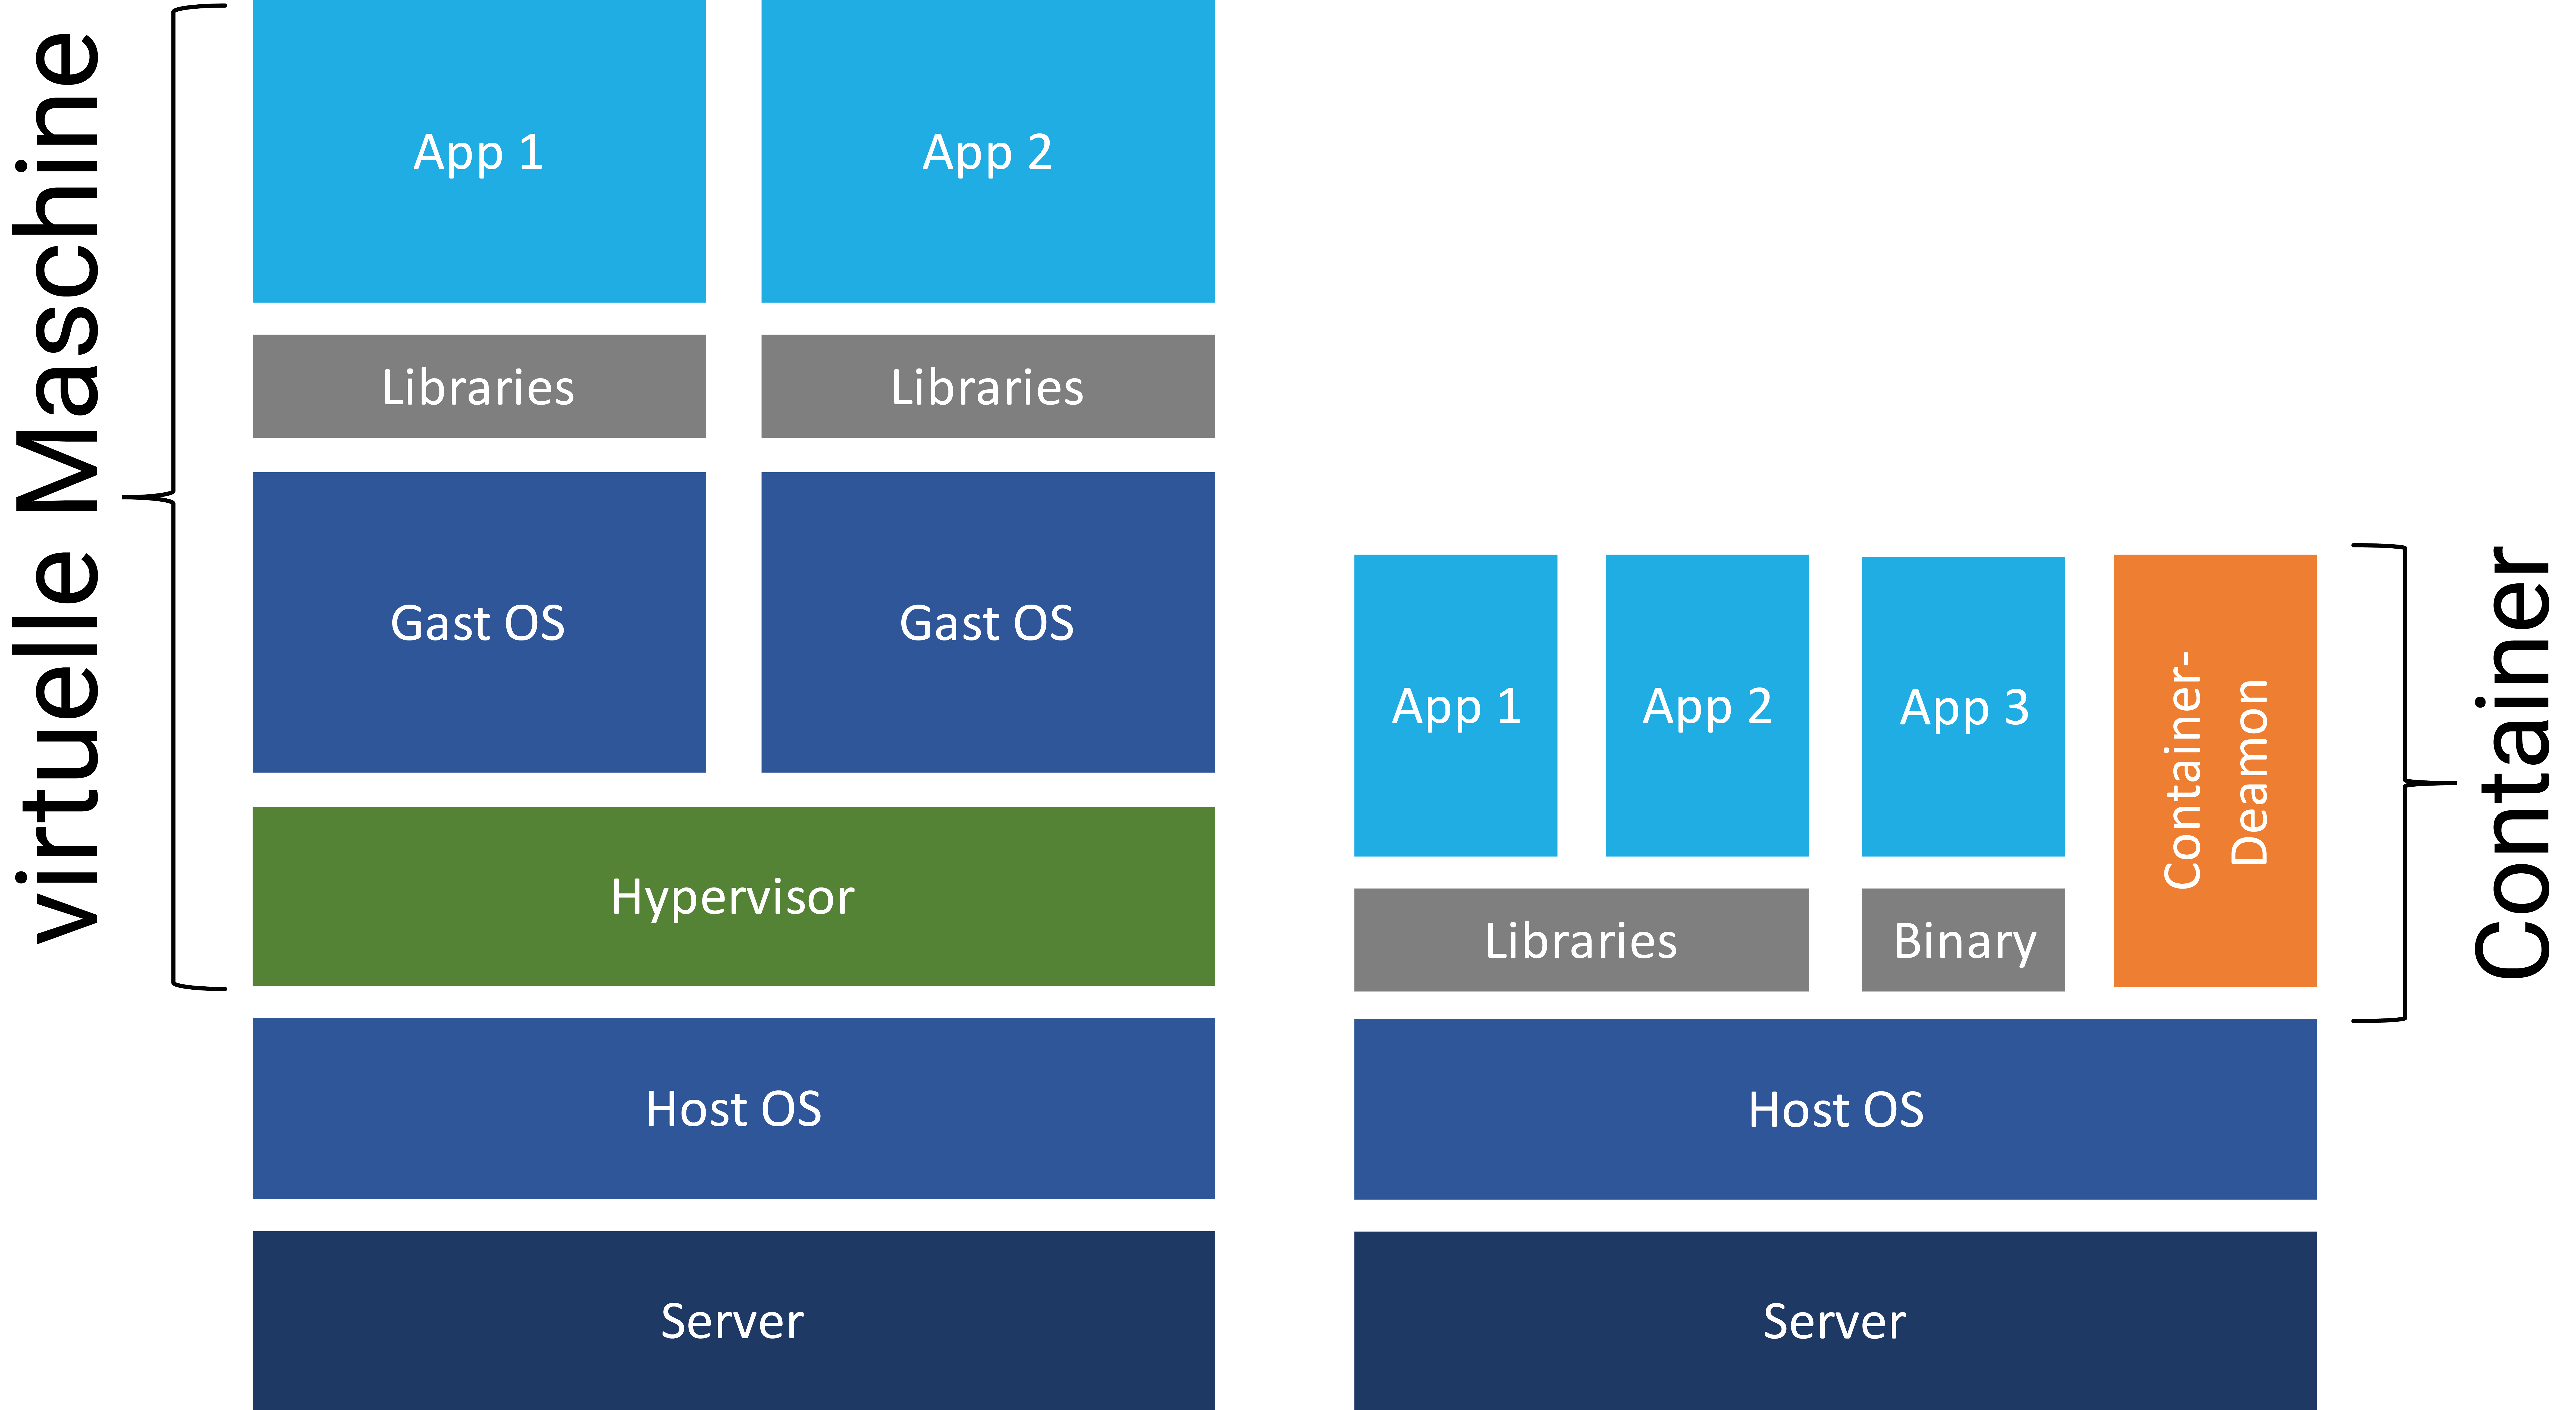
\includegraphics[width=1\textwidth]{VMvsCont.png}
	\end{center}
	\caption[Vergleich Container und VM]{Vergleich Container und VM}
	\label{fig:VergleichContainerVM}
\end{figure}
\newpage



%\input{Inhalt/Funktionalität}
%% !TEX root = ../Ausarbeitung.tex
\section{Containertechnologien} 
\label{sec:Containertechnologien}

In der Geschichte der Containertechnologie traten verschiedene Implementierungsformen auf.
Hierbei waren die ersten Umsetzungen noch sehr einfach aufgebaut und wurden mit den Anforderungen an die Containerdienste immer komplexer.
Im Folgenden findet sich eine Übersicht über die wichtigsten Technologien der Containerisierung.

\begin{figure}[H]
	\begin{center}
		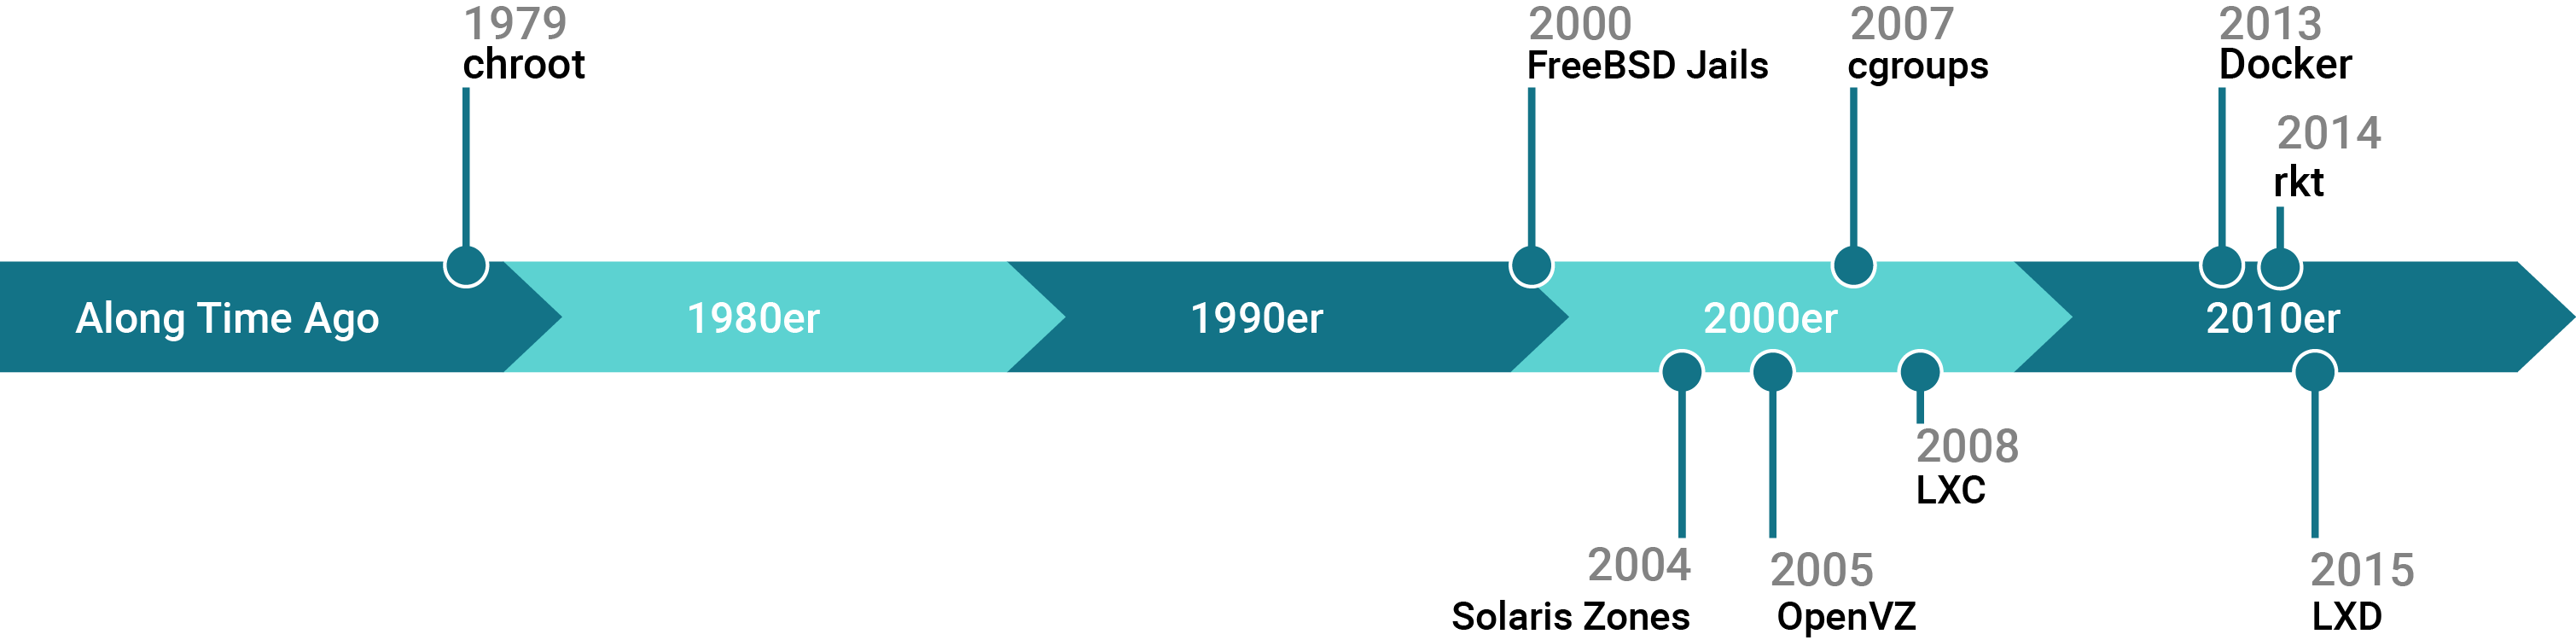
\includegraphics[width=1\textwidth]{ZeitContainer.png}
	\end{center}
	\caption[Containertechnologie im Laufe der Zeit]{Containertechnologie im Laufe der Zeit}
	\label{fig:CTZeit}
\end{figure}


\subsection*{chroot}
\label{sec:chroot}

Chroot ist ein Befehl, der schon früh in Unix-Systemen eingebaut wurde.
Er ermöglicht es, einem Prozess ein anderes Rootverzeichnis zu geben.
Wird in einem Programm \code{chroot()} aufgerufen, wechselt es das Verzeichnis und kann nicht auf Dateien außerhalb der zugewiesenen Struktur zugreifen.
Diese Abschottung eines Prozesses war nie als Sicherheitsfeature vorgesehen und wird hauptsächlich zur Virtualisierung eingesetzt.
Mit dem Befehl können einzelne Prozesse auf Dateiebene von anderen Anwendungen getrennt werden, weitere Sicherheitsmechanismen oder Isolierungen gibt es nicht. \citep{IEEE7830207,569694, MANPAGE01}
\newpage
\subsection*{OpenVZ}
\label{sec:OpenVZ}

\begin{wrapfigure}{l}{0.4\textwidth}
	\vspace{-40pt}
	\begin{center}
		
\includegraphics[width=0.3\textwidth]{openvz.png}
	\end{center}
	\vspace{-15pt}
	\caption[Logo OpenVZ]{Logo OpenVZ \footnotemark}
	\label{fig:openvz}
	\vspace{-30pt}
\end{wrapfigure}
\quellefoot{https://upload.wikimedia.org/wikipedia/commons/b/bb/OpenVZ-logo.png?download}

Im Jahr 2005 veröffentlichte die Firma SWsoft (später umbenannt zu Parallels) ihr Projekt OpenVZ unter der GNU GPL Lizenz. OpenVZ basierte auf der Idee der Container, ermöglicht es jedoch in jedem Container eine eigene Linux-Distribution auszuführen.
Die durch die Containerumgebung abgegrenzten Betriebssysteme teilen sich einen Kernel. Dadurch ist der Overhead von OpenVZ deutlich geringer als bei der klassischen Vollvirtualisierung eines Betriebssystems.
In den einzelnen Containern gibt es jeweils einen eigenen root-User und eine eigene Dateistruktur.
Sie können unabhängig voneinander gestartet und gestoppt werden.
Da sich die Betriebssysteme einen Kernel teilen, müssen die Gastsysteme ebenfalls Linux-Systeme sein.
Da viele der Änderungen von OpenVZ den Linux Kernel betreffen, werden regelmäßig Änderungen von OpenVZ-Patches in diesen übernommen. \citep{OpenVzNews, IEEE4803091,OpenVzHist}


\subsection*{FreeBSD Jails}
\label{sec:jails}
Mit der Veröffentlichung von FreeBSD 4.0 im Jahr 2000 war FreeBSD Jails das erste richtige System für Containervirtualisierung.
Die FreeBSD Jails basieren auf dem Konzept von chroot. Auch hier wird das root-Verzeichnis eines Prozesses geändert. Zusätzlich verbessert Jails das Konzept um einige Aspekte. Jede Jail erhält einen eigenen Hostnamen und eine eigene IP-Adresse. Sie hat auch ihre eigenen Benutzer, inklusive einem root-Benutzer. \citep{FreeBSDHB14} Durch diese Prozessisolation ergibt sich eine Art Containersystem. Da die Jails als eigener Prozess laufen, können sie unabhängig voneinander gestartet und gestoppt werden. Jails wird gerne für den Einsatz in Netzwerkaufgaben eingesetzt, da die Performance sehr gut ist. Allerdings besitzt Jails kein so großes Ökosystem wie beispielsweise Docker oder OpenVZ. Daher wird es in der Containervirtualisierung von diesen Gegenspielern verdrängt.


\subsection*{\ac{LXC}}
\label{sec:LXC}
\begin{wrapfigure}{r}{0.4\textwidth}
	\vspace{-40pt}
	\begin{center}
		\includegraphics[width=0.3\textwidth]{LXC.png}
	\end{center}
	\vspace{-15pt}
	\caption[Logo \ac{LXC}]{Logo \ac{LXC} \footnotemark}
	\label{fig:LXC}
	\vspace{-30pt}
\end{wrapfigure}
\quellefoot{https://upload.wikimedia.org/wikipedia/commons/4/40/Linux_Containers_logo.png?download}
\ac{LXC} ist seit der erstmaligen Veröffentlichung 2008 ein offizielles Kernelfeature und in den meisten Distributionen von Linux enthalten. \ac{LXC} ist eine User Space-Schnittstelle für die Erstellung von isolierten Umgebungen innerhalb eines Systems. Dies geschieht durch die Nutzung von Kernel namespaces, Apparmor und SELinux-Profilen sowie chroots und cgroups. Diese Features standen schon vor \ac{LXC} zur Verfügung, jedoch vereinigte sie \ac{LXC} zu einer Schnittstelle für die Erzeugung von Containern. Zu Beginn der Entwicklung von \ac{LXC} war die Isolation der Container nicht gut, sondern glich eher einer Abwandlung der chroot-Funktion. Mit der Zeit wurde die Abschottung jedoch immer besser und die \ac{LXC}-Container wurden zu richtigen virtualisierten Umgebungen. Dies geschah unter anderem dadurch, dass ab Version 1.0 die einzelnen Container als unpriviliegierte Benutzer ausgeführt werden können. Zuvor war dies nicht möglich und eine Abgrenzung der Container nur bedingt gegeben. \ac{LXC} ist eine Technologie, die von vielen weiteren Projekten eingesetzt wird, unter anderem von Proxmox oder Docker (bis Version 1.1)\citep{IEEE7036275, IEEE7185212, IEEE7571957,IEEE7929714,LXCHomepage}


\subsection*{LXD}
\label{sec:lxd}

Um die Verwendung von \ac{LXC} zu vereinfachen, wurde das Tool LXD entwickelt. Es besteht aus drei Elementen: Einem Daemon, der eine REST-API zur Verfügung stellt, einem Befehlszeilenclient sowie einem Open-Stack Nova Plugin. Die vom Daemon bereitgestellte Schnittstelle ermöglicht es, über das Netzwerk auf das Management der Container zuzugreifen. LXD ist somit eine Erweiterung, die eine Schnittstelle zu \ac{LXC}-Containern schafft. Über das Nova Plugin können die einzelnen LXD-Maschinen als Rechenknoten verwendet werden. \citep{LXDHomepage}

\subsection*{Solaris Zones}
\label{sec:solariscontainer}

Im Jahr 2004 veröffentlichte Oracle im Build 51 von Solaris 10 zum ersten Mal ein Feature mit dem Namen Solaris Containers. Solaris Containers stellt eine Technologie dar, mit der auf x86 und SPARC-Systemen Betriebssystemlevelvirtualisierung durchgeführt werden kann. Später zusammengelegt zu Solaris Zones, bestanden die beiden Technologien Solaris Containers und Solaris Zones parallel zueinander. Dabei war Zones eine klassische Virtualisierungsplattform mit Hypervisor und Containers eine Containertechnologie, die analog zu chroot funktionierte. Mit der Zusammenlegung von Containers und Zones zum neuen Zones wurde daraus eine Containerumgebung, in der die Container sicher voneinander und dem Host getrennt sind und von einem Resourcenmanagement kontrolliert werden. \citep{OracleZonesIntro,OracleZonesOver}
	

%\subsection{Windows Containers}
%s\label{sec:WindowsContainers}



\subsection*{Docker}
\label{sec:Docker}


dotCloud veröffentlichte im März 2013 das Projekt mit dem Namen Docker, dieses Projekt stellte Solomon Hykes auf der PyCon 2013 zum ersten Mal der Öffentlichkeit vor. \citep{dockeryout1} Ein paar Monate später kündigte dotCloud Inc. an, den Firmennamen zu Docker Inc. zu ändern und sich hauptsächlich der Entwicklung des Docker Ökosystems zu widmen. \citep{dockerblog} Die Firma Docker Inc. (im Folgenden "`Docker Inc."' oder "`Hersteller"') hat bis zum heutigen Tag das Projekt Docker (im Folgenden "`Docker"') weiterentwickelt und das zugehörige Ökosystem ausgebaut. So wurde unter anderem der DockerHub eingerichtet, eine Plattform um Images zu teilen und auszutauschen. \citep{dockermanual}

Zu Beginn war Docker lediglich eine Werkzeugsammlung um \ac{LXC}-Container zu verwalten. Jedoch baute Docker Inc. diese Sammlung immer weiter aus und erweiterte das System um Funktionen, die vom unterliegenden Linux-Betriebssystem nicht gegeben waren. Mit der Version 0.9 veröffentlichte Docker Inc. den neuen Treiber libcontainer und nutzte ihn ab diesem Zeitpunkt als native Umgebung für Docker-Container. \citep{dockerblog2} Zu Beginn unterstützte Docker lediglich Linux-Container und nutzte dazu unter Windows eine virtuelle Maschine (Windows 7 \& 8) oder das Linux-Subsystem (Windows 10). Ab der Version 17.11 von Docker für Windows und dem Windows 10 Fall Creators Update konnten erstmals Windows Container genutzt werden. \citep{dockerblogwin} Auch entwickelte Docker Inc. weitere Zwischebenen, um sich von \ac{LXC} zu lösen und die Umgebung in Module zu teilen. So entstand containerd, ein Container-Daemon, mit dem die Docker Engine kommuniziert. Dieser Daemon wiederum kann mit einem OCI-konformen Container-Tool umgehen und über dieses Container starten (\Vgl \Abbildung{containerrunc}). Ein solches Tool ist das eigene runC. Auf diese Art können Docker-Container auch durch andere Orchestrierungstools wie Kubernetes oder Swarm verwaltet werden (\Vgl \Abschnitt{Cluster}). \citep{Buch}

\begin{figure}[h]
    \begin{center}
        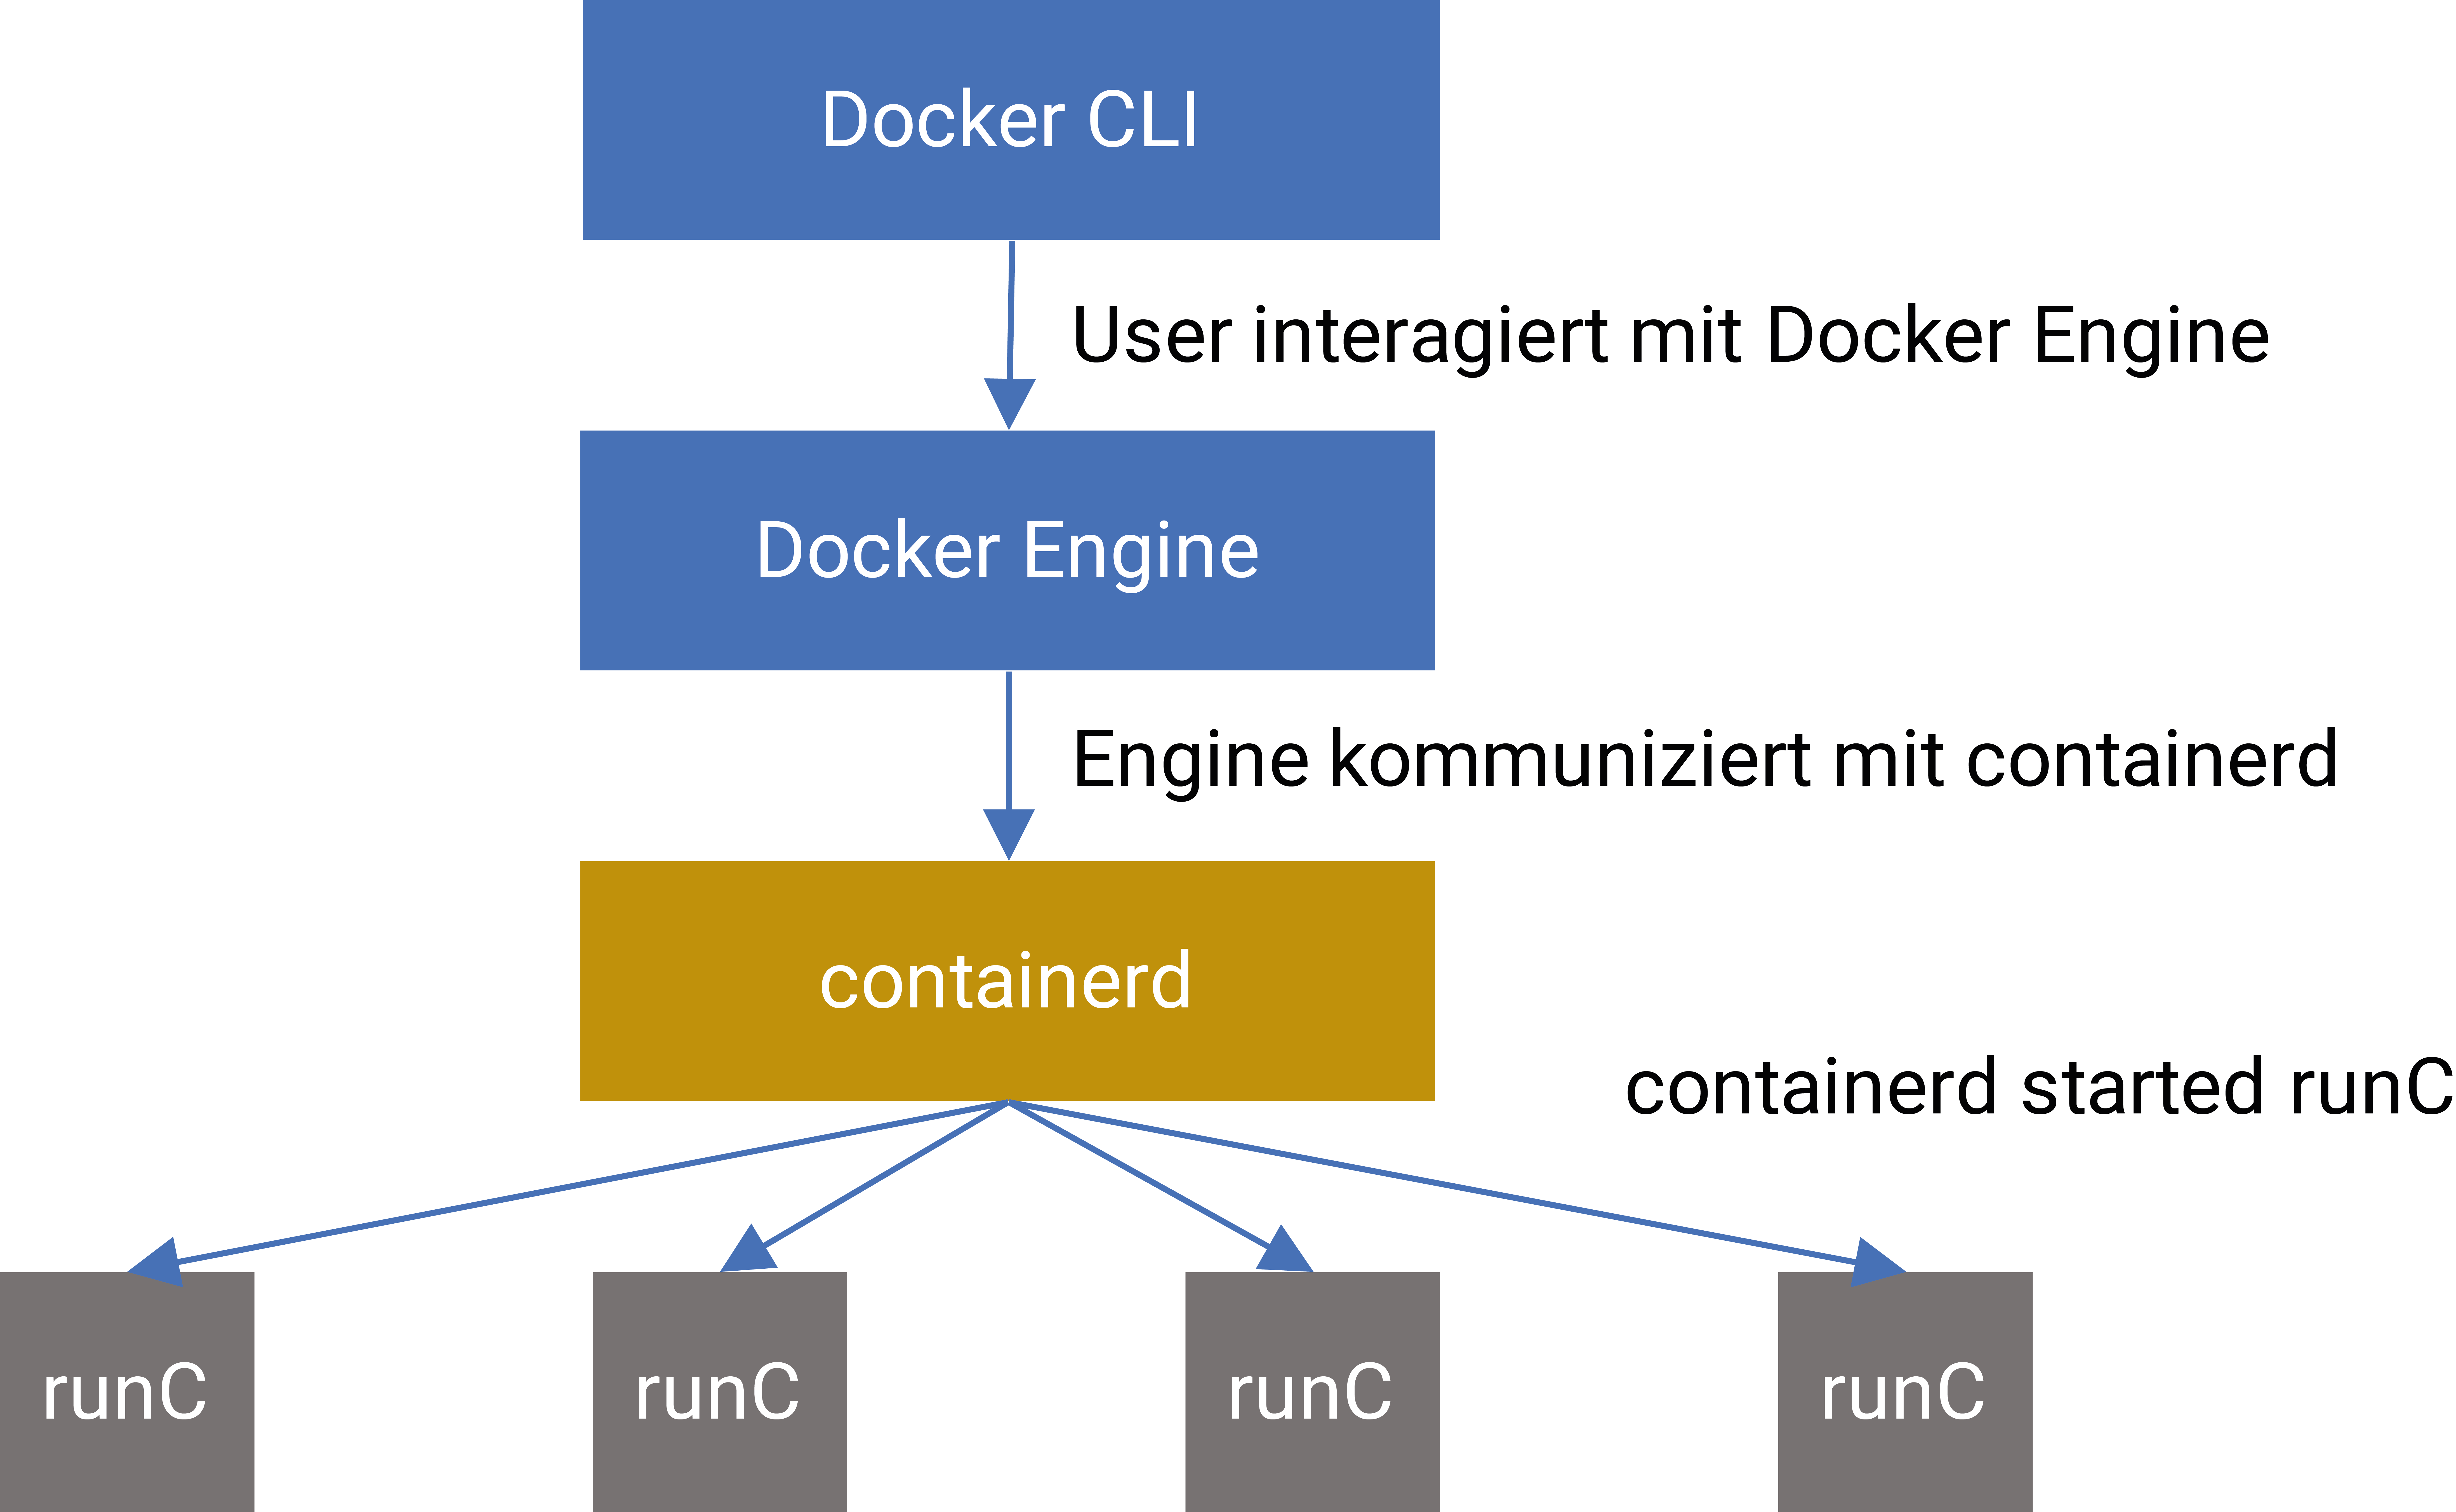
\includegraphics[width=0.6\textwidth]{clitorunc.png}
    \end{center}
    \caption[Kommunikation zwischen Engine und runC]{Kommunikation zwischen Engine und runC}
    \label{fig:containerrunc}
\end{figure}

Zum heutigen Zeitpunkt ist Docker die führende Containerumgebung (\Vgl \Abbildung{Stats2}), daher wird die Funktion derselben im Folgenden anhand eines Beispielcontainers aufgezeigt:

In diesem Beispiel soll innerhalb eines Docker-Containers ein Python-Skript ausgeführt werden. Als Basis für eine Container-Instanz dient ein schreibgeschütztes Image. Dieses enthält alle benötigten Teile des OS abgesehen vom Kernel, denn dieser wird bereits durch den Host zur Verfügung gestellt. Zusätzlich gehören auch benötigte Abhängigkeiten zu einem Image. Auf diesem schreibgeschützten Teil wird dann ein schreibbarer Layer aufgebaut, wenn von dem Image eine Container-Instanz abgeleitet wird. Wird die Container-Instanz beendet, sind alle Änderung innerhalb des schreibbaren Layer verloren. Um die Änderungen zu sichern, kann ein sogenannter Snapshot angelegt werden, der dem Image einen weiteren read-only-Layer hinzufügt. Die Anzahl der Layer ist, je nach Docker-Version, auf 127 beschränkt. \citep{Buch, dockermanual} Der Aufbau des Images unseres Beispielcontainers sieht aus wie in \Abbildung{docker1} dargestellt:

\begin{figure}[h]
    \begin{center}
        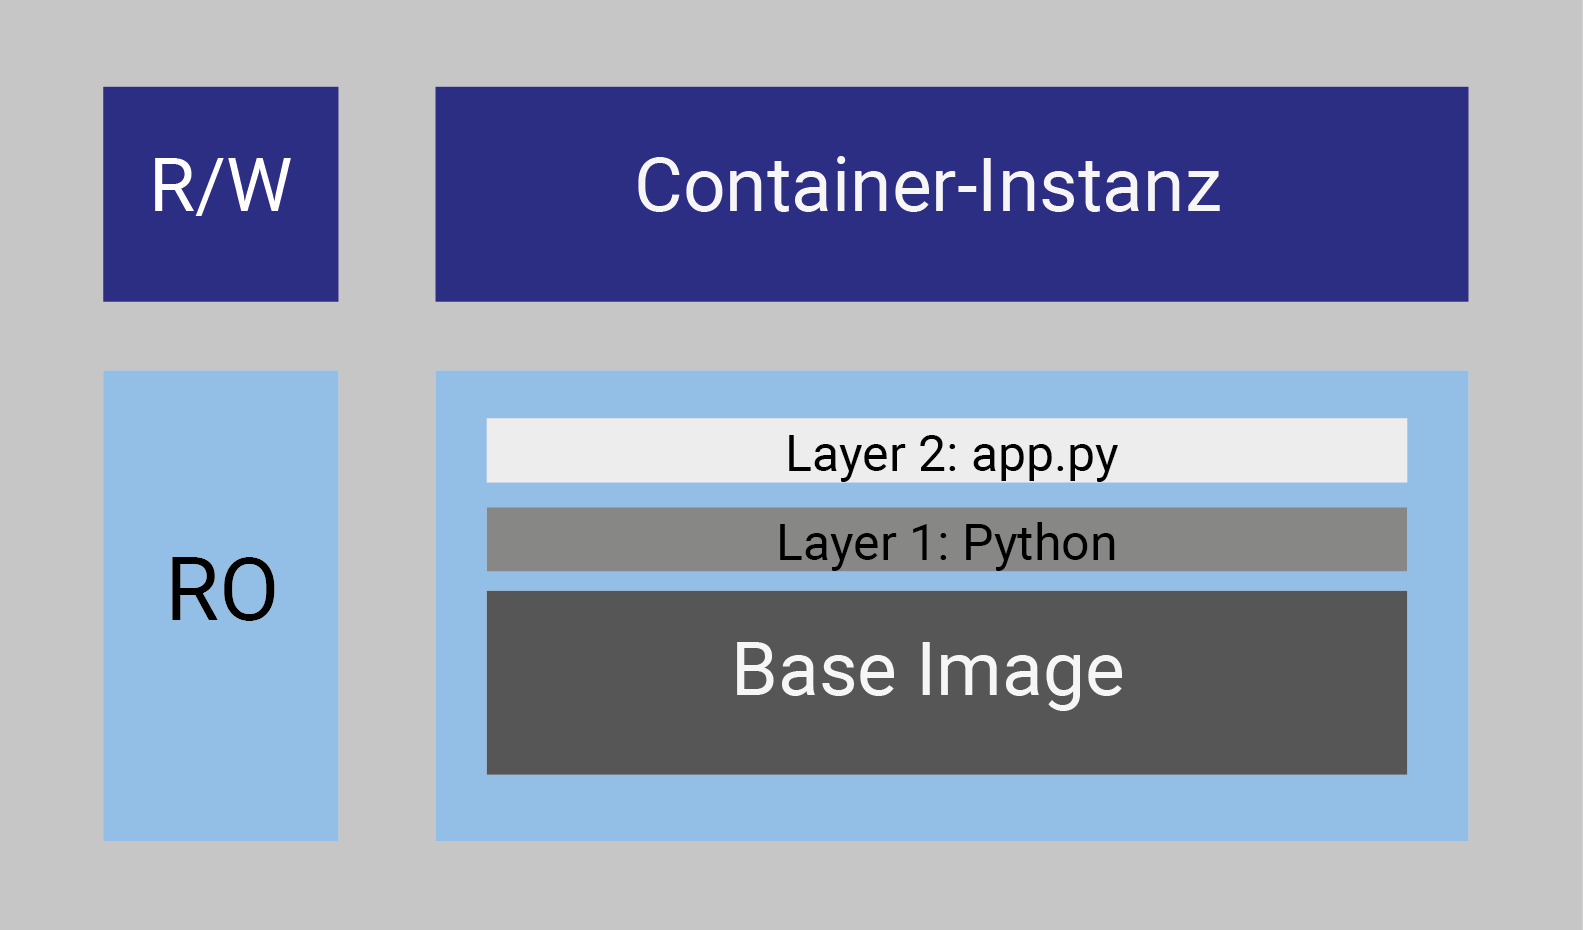
\includegraphics[width=0.6\textwidth]{DockerImage.png}
    \end{center}
    \caption[Image des Beispielcontainers]{Image des Beispielcontainers}
    \label{fig:docker1}
    \end{figure}

Als Basis dient ein Image, in dem Alpine Linux installiert ist. Python wird als weiterer Layer hinzugefügt. Zu diesen Layern wird noch das Python-Skript hinzugefügt. Dies zusammen ergibt dann den schreibgeschützten Teil, von dem die Container-Instanz abgeleitet wird. In dieser legt das Python-Skript Dateien an und schreibt in diese. Wird der Container beendet, werden alle angelegten Dateien verworfen.\\
Der Aufbau des Images kann in einem Dockerfile beschrieben werden. Für unser Beispiel sieht dieses wie folgt aus:

\begin{lstlisting}[language=docker,caption={Dockerfile},label={code:dockerfile}]
FROM python:3 

WORKDIR /usr/src/app

COPY ./app.py ./app.py

CMD ["python", "./app.py"]
\end{lstlisting}

In dem Dockerfile wird zuerst definiert, dass das Image auf dem vorhanden Python-Image aufbauen soll. Dieses wiederum baut auf einem Alpine-Linux-Image auf. Daraufhin wird das aktuelle Arbeitsverzeichnis im Container geändert. Anschließend wird die im Arbeitsverzeichnis des Host abgelegte Datei "`app.py"' in das Arbeitsverzeichnis des Container übertragen und schließlich der Befehl definiert, der beim Start des Containers ausgeführt werden soll. Das Python-Skript legt eine Datei an und gibt deren Dateiname und Inhalt in der Konsole aus:
\begin{lstlisting}[language=python,caption={app.py},label={code:pythonapp}]
#!/usr/bin/python3

print("Ausgabe zur Kommandozeile")
file=open("datei.txt", "a+")
print("Dateiname: ", file.name)
file.write("Eine neue Zeile\n")
file.close()
print(open("datei.txt","r").read())
\end{lstlisting}
Nun kann mit dem Befehl \code{docker build} das Image erstellt werden. Dabei lädt Docker zunächst das Image von python aus dem oben genanten Docker-Hub herunter und legt darauf den Layer mit dem Python-Skript:

\begin{lstlisting}[language=bash,caption={Terminalausgabe docker build},label={code:dockerbuild}]
user@dockerpc:~$ docker build -t pythontest .
Sending build context to Docker daemon 311.4MB
Step 1/4 : FROM python:3
 ---> 638817465c7d
Step 2/4 : WORKDIR /usr/src/app
---> 8d3ab23442c9
Step 3/4 : COPY ./app.py ./app.py
---> 2b0882cadee4
Step 4/4 :  CMD ["python", "./app.py"]
---> 5a8a392a0856
Successfully built 5a8a392a0856
Successfully tagged pythontest:latest
\end{lstlisting}

Nun liegt das Image bereit und es kann ein Container davon abgeleitet werden. Dazu reicht der einfache Befehl \code{docker run}, um den Container zu starten:

\begin{lstlisting}[language=bash,caption={Terminalausgabe docker run},label={code:dockerbuild}]
user@dockerpc:~$ docker run pythontest
Ausgabe zur Kommandozeile
Dateiname: datei.txt
Eine neue Zeile
\end{lstlisting}

Hier wird nun das Python-Skript in dem Container ausgeführt und der Container daraufhin beendet und somit auch die beschriebene Datei gelöscht. Wird der Container erneut ausgeführt, so wird eine neue Datei erstellt:

\begin{lstlisting}[language=bash,caption={Terminalausgabe docker run mehrfach},label={code:dockerbuild}]
user@dockerpc:~$ docker run pythontest
Ausgabe zur Kommandozeile
Dateiname: datei.txt
Eine neue Zeile

user@dockerpc:~$ docker run pythontest
Ausgabe zur Kommandozeile
Dateiname: datei.txt
Eine neue Zeile
\end{lstlisting}

Die Layer, aus denen Docker die verschiedenen Images aufbaut wurden von Docker Inc. in den ursprünglichen \ac{LXC}-Container hinzugefügt und später in den libcontainer übernommen. Durch diese Layer ist es einfacher Ressourcen zu teilen. Wenn mehrere Images auf Python oder Alpine-Linux aufbauen sollen, so müssen diese beiden Ressourcen nicht mehrfach heruntergeladen werden, sondern stehen jedem Image zur Verfügung. Dies ist einer der Gründe, warum Docker nach der Veröffentlichung große Popularität erreichte und heute die führende Containertechnologie ist. \citep{dockermilestones}



\subsection*{rkt}
\label{sec:rkt}

\begin{wrapfigure}{l}{0.4\textwidth}
	\vspace{-40pt}
	\begin{center}
		
\includegraphics[width=0.3\textwidth]{rkt.png}
	\end{center}
	\vspace{-15pt}
	\caption[Logo rkt]{ \footnotemark}
	\label{fig:rkt}
	\vspace{-30pt}
\end{wrapfigure}
\quellefoot{https://github.com/rkt/rkt/raw/master/logos/rkt-horizontal-color.png}


rkt (Ausprache wie "rocket") ist eine Containerengine, die sich als Alternative zu Docker etabliert hat und von CoreOS veröffentlicht wurde und weiterentwickelt wird. Das Open-Source-Projekt ist unter der Apache License 2.0 veröffentlicht. \citep{RepoRkt} Unter rkt werden viele Grundgedanken von UNIX umgesetzt. Z.B. liegen alle Container als Dateien vor, die einfach verwaltet werden können. Auch legt rkt einen großen Wert auf Sicherheit und setzt dazu verschiedene Techniken ein, die inzwischen von den meisten Konkurennten übernommen wurden. So kann rkt für jeden Container entscheiden, ob dieser auf Basis von KVM oder einer virtuellen Maschine isoliert wird und führt alle Prozesse, auch den Download von Images, als nicht priviligierter Benutzer aus. In rkt wird die kleinste Einheit Pod genannt. Sie kann aus einem oder mehreren Containeren bestehen, welche sich die Ressourcen teilen. So passt das Konzept von  rkt direkt zu den Konzepten von  Cluster-Managern. Auch besitzt rkt keinen zentralen Service, der alle Container überwacht, sondern arbeitet direkt mit dem systemeigenen systemd zusammen, um die Container zu verwalten. Somit lässt sich rkt auch direkt mit Kubernetes verknüpfen, für das der Herausgeber von rkt, CoreOS, die kommerzielle Implementierung Tectonic entwickelt. rkt unterstützt auch die Konvertierung von Docker-Containern zu rkt-Pods. \citep{HomepageRkt,ixrkt}


%% !TEX root = ../Ausarbeitung.tex
\section{Container in der Softwareentwicklung} 
\label{sec:Softwareentwicklung}

Der Einsatz von Containern erleichtert die Entwicklung von Software in vielerlei Hinsicht. So müssen Entwickler ihre Applikationen für verschiedene Plattformen nicht grundlegend verschieden entwerfen und die Programmiersprache kann meist frei gewählt werden. 
Ob für Windows, Linux, MacOS, Cloud-Plattformen oder andere, der Fokus der Entwicklung kann deutlich stärker auf die Funktionalitäten der Applikation gerichtet werden, wenn die Eigenheiten der Ziel-Plattform in den Hintergrund rücken. Das macht den gesamten Entwicklungsprozess einfacher und somit effizienter.
Mithilfe der Abstraktion durch Container vermeidet man Inkompatibilitätsprobleme auf den Host-Geräten und auch die Entwicklung sowie Softwaretests gestalten sich dadurch leichter, schneller und effizienter, denn alle für die Applikation wichtigen Daten, Tools und Systembibliotheken sind im Container vorhanden.
\citep{11517836120160501}

Entwickler können davon ausgehen, dass ihre Applikation auf verschiedenen Systemen funktionieren wird und können sie immer unter konsistenten Bedingungen testen, egal wie später die Umgebung aussehen mag. Dies erhöht die Zuverlässigkeit enorm. Man ist nicht länger abhängig von der Verfügbarkeit von identischen Entwicklungs- und Testsystemen und der Entwickler kann auf seinem eigenen Rechner auch schnelleres Feedback erhalten, wenn er den Container lokal ausführt und debuggt.

Auch ermöglichen Container die Verwendung von Microservices. Sonst als monolithische Applikation entworfene Software kann von Entwicklern unabhängig in mehreren Teilen erstellt werden, was die Agilität deutlich fördert.
Außerdem ist das Software Deployment sehr simpel, da es nur gilt, ein Container Image zu erzeugen und zu verteilen. Dies kann auch über Container-Orchestration-Tools wie Kubernetes nach dem Prinzip von Continous Delivery automatisiert werden. Die Ausführung läuft auf jedem System dann jedes Mal identisch ab.
\citep{ItAgil}

Dementsprechend benötigt man auch für Weiterentwicklung und Wartung der Applikationen weniger Zeit und Personal als wenn man für jedes System eigene Entwickler mit Fachkenntnissen bräuchte.
Bei Veränderungen an der Hardware, kurzfristigem Wechsel, Neuanschaffungen aber auch bei Upgrades des Betriebssystems hat eine Firma keine größeren Schwierigkeiten durch Inkompatibilitäten zu befürchten. Somit ist sie auch freier in der Wahl ihrer Geräte.

Auch das sogenannte Monitoring, die laufende Überwachung der Systeme, über Schnittstellen (APIs) ist mit Containern kein Problem. Logs können von jeder Applikation erstellt, dann einfach gesammelt und in ein Management-System übertragen werden. Die Erkennung und Eingrenzung von Fehlerquellen beschleunigt sich dadurch, dass die Applikation im Container gekapselt ist und keine weiteren Programme oder Betriebssystemteile die Fehlersuche erschweren. Auch können die Container-Applikationen einfach mit ihrem vordefinierten Idealzustand neugestartet werden, sobald ein Problem erkannt wird.
Diese Vereinfachung durch Abstraktion hilft dann nicht nur dem Entwickler, sondern trägt zur Zufriedenheit der Nutzer bei. 

Besonders wenn es darum geht, neue Applikationen zu entwerfen, deren Zielplattformen noch nicht endgültig festgelegt sind, oder bei einem Umzug in die Cloud. Gerade bei Cloud-Diensten sind Container unter anderem wegen ihres geringeren Ressourcen-Umfangs beliebt.
\citep{12771285120180201}

"Container eignen sich optimal für dienstbasierte Architekturen. Im Gegensatz zu monolithischen Architekturen, bei denen alle Teile einer Anwendung miteinander verknüpft sind […], werden diese Komponenten bei einer dienstbasierten Architektur getrennt. Durch eine Trennung und Arbeitsteilung werden Ihre Dienste auch dann weiter ausgeführt, wenn andere fehlschlagen. Damit bleibt Ihre gesamte Anwendung zuverlässiger."\citep{GoogleContainers}

Tools, die sich speziell um das Ressourcen-Management kümmern, sind in vielen Containern mit inbegriffen, sodass beispielsweise der zur Verfügung stehende Speicher sinnvoll begrenzt werden kann, um Out-of-Memory-Abstürzen vorzubeugen. 
Das schont die Server, auf denen die Applikationen laufen, und reduziert den Hardware-Bedarf und die Kosten, wenn weniger virtuelle Maschinen mit eigenem vollwertigen Betriebssystem aufgesetzt werden müssen.
\citep{11517836120160501}
%% !TEX root = ../Ausarbeitung.tex
\section{Cluster}
\label{sec:Cluster}
Wie in \Abschnitt{Einleitung} genannt, wurden in der Vergangenheit dedizierte Server für jeweils einen Service genutzt.
Dies hatte den Nachteil einer geringen Serverauslastung sowie bei nicht redundanten Servern die Gefahr eines Totalausfalls eines Services.
Applikationen ließen sich nicht ohne weiteres von einem Server auf einen anderen umziehen, da sie tief in das Hostsystem integriert waren.

Cluster Manager verbinden mehrere Maschinen zu einer Einheit. Während Lösungen wie Apache Mesos eine Abstraktion der Hardware vornehmen, basieren Kubernetes und Docker Swarm auf der Container-Architektur.
Diese Cluster Manager übernehmen die Verwaltung der Container sowie ihre Zuordnung zu den jeweiligen Maschinen.

Clustering sorgt für eine verbesserte Redundanz und erhöht somit die Ausfallsicherheit.
Außerdem lässt sich so eine bessere Ressourcen-Allokation vornehmen.

Thema aktueller Forschungsarbeiten ist die Verbesserung des Schedulings, um die Ressourcennutzung zu optimieren. \citep{Liu2018}


%% !TEX root = ../Ausarbeitung.tex
\section{Risiken der Containertechnologie}
\label{sec:Risiken der Containertechnologie}
% Einleitung mit Fragestellung
Die Containertechnologie erobert in den letzten Jahren immer mehr die Rechenzentren. Doch welche Risiken verbergen sich dahinter und wie kann man sich schützen?

% Multiplizierung von Sicherheitslücken
Durch die hohe Anzahl an Containern pro Server ist das Risiko bei einer Sicherheitslücke deutlich höher, da sich diese dann in beispielsweise 80 Containern, anstatt in vier virtuellen Maschinen oder einem dedizierten Server ausnutzen lässt.

% Risiko infizierter Images
Um sich den Aufwand für die Konfiguration der Images zu sparen (diese kann sehr aufwendig sein), verwenden viele Administratoren vorgefertigte Container-Images aus einem Respository.
Dabei muss dem Ersteller vertraut werden, dass das Image keinen Schadcode oder Hintertüren enthält, da der Aufwand für eine genaue Prüfung des Container-Inhalts sehr aufwendig wäre.
Im Juni 2018 hatte die Sicherheitsfirma Kromtech berichtet, dass über das Repository Docker Hub mehrere Images über ein Jahr lang verfügbar waren, die Schadcode zum Minen von Kryptowährungen enthielten.
Diese wurden insgesamt fünf Millionen mal installiert, bevor die Betreiber von Docker Hub reagierten und diese entfernten.
\citep{kromtech}
Die betroffenen Administratoren hätten das Risiko minimieren können, indem Sie nur Container von dem offiziellen Docker Repository bezogen hätten.
Dort werden Images vor ihrer Veröffentlichung geprüft.
\citep{DockerHubOfficial}
Ein Angreifer müsste zur Verteilung eines infizierten Images den Schadcode verstecken, sodass er bei der Prüfung nicht sichtbar wird. Dies stellt eine wesentlich höhere Hürde dar.

% Schnittstellen zum Kernel
Werden Applikationen in Containern richtig verpackt, so sind die einzigen Abhängigkeiten nach außen hin die Systemaufrufe des Betriebssystems.
Dies verbessert die Portabilität der Anwendungen ungemein, allerdings sind auch Systemaufrufe wie z.B. Socket-Schnittstellen sowie hardwarespezifische Systemaufrufe nicht auf allen Systemen einheitlich, wodurch die Portabilität eingeschränkt wird.
Die Open Container Initivative der Linux Foundation arbeitet neben einem Standard für Container Formate auch an einem Standard für Container Runtimes.
Dieser könnte helfen, die Schnittstelle zwischen Container und Betriebssystem besser festzulegen.

% Probleme mit Hardware
Container können nicht gegen Einflüsse schützen, die nicht vom Betriebssystem verwaltet werden. Hierzu sind virtuelle Maschinen als zusätzliche Sicherheitsschicht ratsam. \citep{11517836120160501}

% Prozessorprobleme
Nicht zuletzt haben die Sicherheitslücken Meltdown \citep{DBLP:journals/corr/abs-1801-01207} und Spectre \citep{DBLP:journals/corr/abs-1801-01203} gezeigt, dass über Sicherheitslücken in Prozessoren containerübergreifende Angriffe auf Applikationen möglich sind. Hiergegen schützten auch virtuelle Maschinen nicht.  

%% !TEX root = ../Ausarbeitung.tex
\newpage
\section{Aktuelle Lage}
\label{sec:AktuelleLage}
\Abbildung{Stats1} zeigt, dass trotz einiger Risiken der Container Technologie Unternehmen weltweit immer mehr Geld in die Containerisierung ihres Unternehmens investieren. Laut einer Umfrage, welche auf der DockerCon durchgeführt wurde, investierten 32\% der Unternehmen mindestens 500.000\$ jährlich, um die Containerisierung in ihrer Organisation voranzutreiben. \citep{Investments}
\begin{figure}[H]
	\begin{center}
		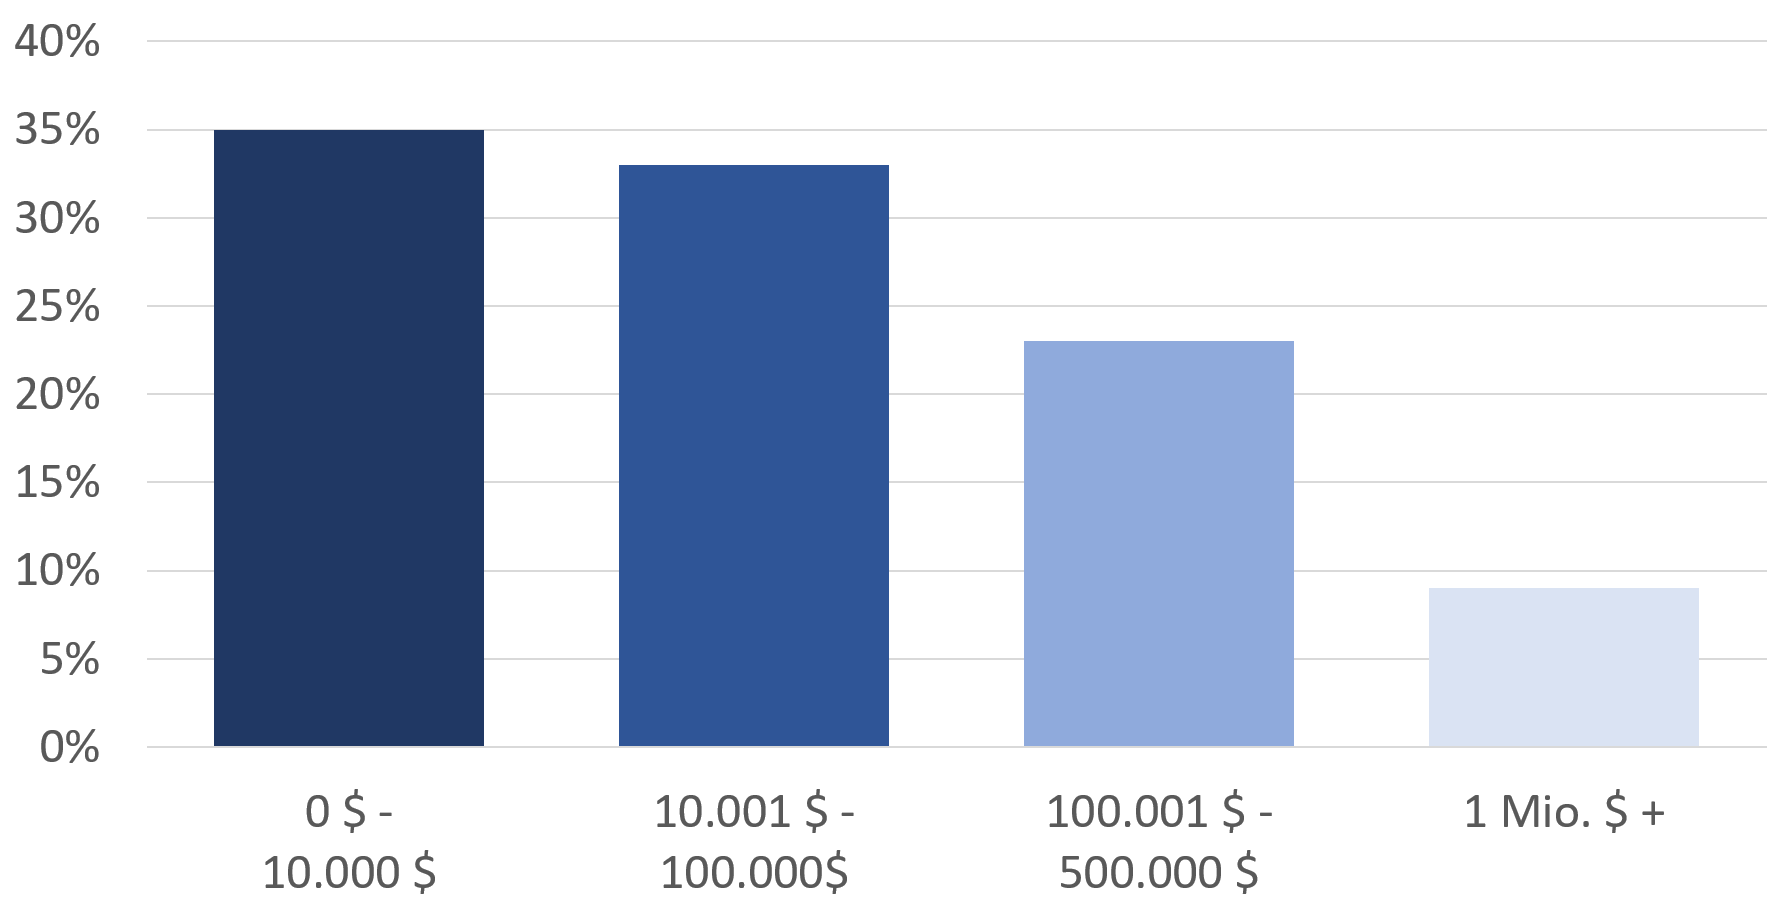
\includegraphics[width=0.8\textwidth]{ContainerInv.png}
	\end{center}
	\caption[Investitionen in die Containerisierung]{Investitionen in die Containerisierung}
	\label{fig:Stats1}
\end{figure}

\newpage
Aus \Abbildung{Stats2} ist zu entnehmen, dass 83\% der produktiv eingesetzten Container von Docker stammen. An zweiter Stelle der meist verwendeten Container findet sich CoreOS, welches von der Firma Red Hat übernommen wurde. Mesos Containerizer und \ac{LXC} machen zusammen nur 5\% aller eingesetzten Container aus. \citep{stats}
\begin{figure}[H]
	\begin{center}
		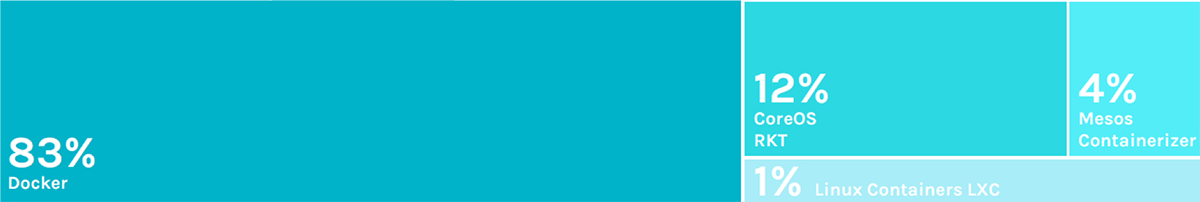
\includegraphics[width=1\textwidth]{DockerProzent.png}
	\end{center}
	\caption[Benutzung von Containertechnologien]{Benutzung von Containertechnologien \footnotemark}
	\label{fig:Stats2}
\end{figure}
\quellefoot{https://www.dailyhostnews.com/wp-content/uploads/2018/05/d2.png}
Laut eines Berichts der Container-Monitoring-Firma Sysdig stieg die Anzahl der durchschnittlich verwendeten Container pro Host 2018 um 50\% im Vergleich zum Vorjahr. Das entspricht nun etwa 15 Containern. Laut des Berichts ist 154 die höchste Anzahl von Containern, die bisher gleichzeitig auf einer Maschine laufen. \citep{stats} \Abbildung{Stats3} stellt dies grafisch dar.
\begin{figure}[H]
	\begin{center}
		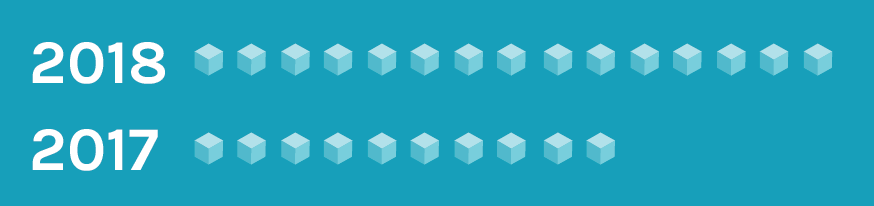
\includegraphics[width=0.8\textwidth]{ContainerHost.png}
	\end{center}
	\caption[Container je Maschine]{Container je Maschine \footnotemark}
	\label{fig:Stats3}
\end{figure}
\quellefoot{https://www.dailyhostnews.com/wp-content/uploads/2018/05/d1.png}
\newpage
Kubernetes sei die meist genutzte Plattform, um Container zu orchestrieren und wird von Software-Unternehmen wie Microsoft und IBM verwendet. Das beliebteste Tool, um Container-Cluster für große Firmen auszurollen, sei jedoch Mesos Containerizer. \citep{stats} Die genaue Verteilung ist \Abbildung{Stats4} zu entnehmen.
\begin{figure}[H]
	\begin{center}
		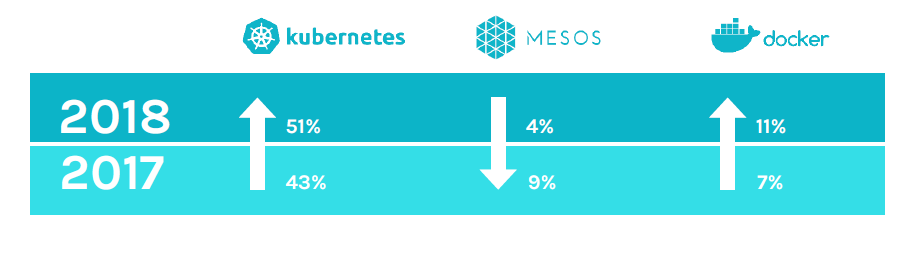
\includegraphics[width=0.8\textwidth]{Manager.png}
	\end{center}
	\caption[Cluster-Manager]{Cluster-Manager \footnotemark}
	\label{fig:Stats4}
\end{figure}
\quellefoot{https://www.dailyhostnews.com/wp-content/uploads/2018/05/d4.png}


%% !TEX root = ../Ausarbeitung.tex
\section{Einsatzszenarien von Containern an der Hochschule}
\label{sec:HS}
Im Folgenden soll betrachtet werden, welche Einsatzmöglichkeiten sich für Container in der IT-Infrastruktur der Hochschule Albstadt-Sigmaringen anbieten und welche Vorteile dies mit sich bringen würde. 

Da Container keine Schnittstelle für grafische Oberflächen bieten, sind die Server-Dienste der Hochschule für den Einsatz prädestiniert.
Hier wäre denkbar den in \Abschnitt{Cluster} vorgestellten Ansatz eines Serververbunds in Verbindung mit einem Cluster Manager wie Docker Swarm oder Kubernetes zu verwenden.
Die einzelnen Applikationen wie z.B. das E-Learning System Ilias, die CentOS Instanzen, die Bibliotheksdienste und die Webserver könnten dann in mehreren Container-Instanzen laufen.
Der Cluster-Manager würde dynamisch die Last auf die verschiedenen Maschinen verteilen und könnte Instanzen mit Programmfehlern erkennen sowie schnell neustarten.

Außerdem wäre es möglich Lastspitzen abzufangen, indem Serverkapazitäten anderer Bildungseinrichtungen genutzt werden, um dort bei Bedarf Containerinstanzen zu starten.

\textbf{Beispiel:}\newline
Ein konkreter Anwendungsfall für die Hochschule Albstadt-Sigmaringen ist die Containerisierung der Oracle Datenbank. Die Datenbank wird im Rahmen mehrerer Vorlesungen und Praktika von Professoren und Studenten genutzt.
Dabei ist die Zahl der Zugriffe auf die Datenbank außerhalb von Vorlesungen oder Praktika sehr gering.
Während Praktika und Vorlesungen wird die Datenbank rege genutzt, wodurch die Performance spürbar leidet.
Dieser starke Unterschied der benötigten Leistung könnte perfekt durch Containerisierung der Datenbank ausgeglichen werden, da je nach Nachfrage innerhalb von Sekunden Container hoch- oder runtergefahren werden können.
Diese Vorgehensweise spart nicht nur Strom, sondern garantiert auch Professoren und Studierenden eine gute Performance der Datenbank. Oracle bietet im Docker Store ein vorgefertigtes Docker Image an, was die Nutzung von Oracle auf Docker sehr vereinfacht.
Eine detaillierte Anleitung für die Containerisierung von Oracle Datenbanken findet man auf der Oracle Homepage\footnote{\url{https://apex.oracle.com/pls/apex/germancommunities/dbacommunity/tipp/6241/index.html}}.
Um die Leistungsfähigkeit der Datenbank weiter zu optimieren, könnte ein in \Abschnitt{Cluster} vorgestellter Cluster-Manager verwendet werden.

%% !TEX root = ../Ausarbeitung.tex
\newpage
\section{Fazit und Ausblick} 
\label{sec:Fazit}
% Aktuelle Lage
In den letzten Jahren stieg die Nutzung von Containern rasant an und viele Unternehmen investieren massiv in diese Technologie (vgl. \Abschnitt{AktuelleLage}). 
Die ausschlaggebenden Gründe hierfür sind der verringerte Overhead, die Performance-Vorteile und das vereinfachte Deployment von Anwendungen. 

% Softwareentwicklung
Im Bereich der Softwareentwicklung bringen Container einen großen Vorteil. 
Es ist möglich innerhalb von Sekunden ein System mit den nötigen Eigenschaften aufzusetzen, um die Anwendung darauf auszuführen. 
Außerdem kann so sichergestellt werden, dass Test- und Produktivsystem absolut identisch sind und keine unerwarteten Effekte auftreten. 

% Business
Durch die immer simpleren Containertechnologien können Unternehmen mit wenig Budget und Personal die Containerisierung ihres Unternehmens vorantreiben und die Vorteile dieser ausschöpfen. 
Somit ist auch in den nächsten Jahren mit dem vermehrten Einsatz von Containertechnologien im Businessbereich zu rechnen. 

% Container und VMs
Allerdings haben Container auch Schwächen, wie z.B. die vorhandenen Abhängigkeiten vom Betriebssystem.
Daher sind sie kein Ersatz für virtuelle Maschinen. Vielmehr ist es ratsam, die beiden Technologien in Kombination miteinander zu verwenden. 
Dabei ist es vor allem zu empfehlen den Docker-Host zu virtualisieren, sodass dieser bei einem Hardwareausfall trotzdem weiter laufen kann und bei Wartungen der Dienst weiter zur Verfügung steht. 
Somit können die in \Abschnitt{Einleitung} genannten Vorteile genutzt werden.

% Container Technologien
Durch die Diversität bei den Containertechnologien können die Anwender Container auf den verschiedensten Betriebssystemen nutzen.
Zudem wird durch die Konkurrenz der Technologien untereinander die Weiterentwicklung und Optimierung der Technik gefördert. 
Auch wurde die \ac{OCI} gegründet, um die Technologie zu standardisieren und eine gemeinsame Weiterentwicklung zu fördern.




\section{Einleitung}
\subsection{Projektbeschreibung}
Im Januar 2020 wird in den USA ein Gesetz in Kraft treten. Dieses verpflichtet die Firma T dazu, alle Schiffscontainer mit einem Tracking-Gerät auszustatten. Dieses Gerät muss die Position des entsprechenden Container über die letzten 9 Monate dokumentieren. Unsere Geräte CONTRAC mit der zugehörigen Software CONSERV bietet diese Möglichkeit. Aus diesem Grund hat uns KT beauftragt die Container des Schiffs "`Event Horizon"' mit unserem System auszustatten. Um die Anforderungen der Firma KT zu erfüllen müssen diese Geräte allerdings mit ZigBee ausgestattet werden und die Software entsprechend erweitert werden. Auch übernehmen wir die Verwaltung des Servers CONSERV für KT.
\section{Annahmen}
\subsection{Sitze und Örtlichkeiten}
\begin{enumerate}
    \item Der Sitz der Firma EZ ist Hamburg
    \item Der Sitz der Firma DOTDAT GmbH ist Hamburg
    \item Der bei KT beschäftigte Projektleiter Lars Haekinson arbeitet in Hamburg
\end{enumerate}

\subsection{Geräte und Anwendungen}
\begin{enumerate}
    \item Die Firma EZ besitzt einen Vorrat von ca. 100 CONTRAC-Geräten für Test- und Entwicklungszwecke in Hamburg
\end{enumerate}

\subsection{Lieferzeiten}
\begin{enumerate}
    \item Die Lieferung großer Frachten aus Shenzhen dauert 40 Tage.
    \item Die Lieferung kleiner Mengen per Luftfracht dauert 5 Tage.
\end{enumerate}

\section{Projektinhalt}
\subsection{Aktivitäten}
\begin{table}[H]
    \renewcommand{\arraystretch}{1.05}
    \begin{center}
        \begin{tabular}{l|l}
            \hline
            \textbf{ID} & \textbf{Aktivität}\\\hline
            A    & Projektmanager                                      \\ \hline
            A1   & Ausführungen                                        \\ \hline
            A2   & Reviews                                             \\ \hline
            A3 & Kommunikation \\\hline
            B    & CONTRAC                                             \\ \hline
            B1   & Entwicklung Verbesserung Hardware (ZigBee und Akku) \\ \hline
            B2.1 & Produktion beauftragen                              \\ \hline
            B2.2 & Produktion                                          \\ \hline
            B3.1 & QS Shenzhen                                         \\ \hline
            B4.1 & Versand                                             \\ \hline
            B3.2 & QS Hamburg                                          \\ \hline
            B4.2 & Versand Rotterdam                                   \\ \hline
            B5.1 & Anbauer Suchen                                      \\ \hline
            B5.2 & Anbau entwerfen                                     \\ \hline
            B5.3 & Anbau testen                                        \\ \hline
            B5.4 & Anbau vorstellen                                    \\ \hline
            B5.5 & Anbau verbessern                                    \\ \hline
            B5.6 & Anbauteile bestellen                                \\ \hline
            B5.7 & Anbau                                               \\ \hline
            C    & CONSERV                                             \\ \hline
            C1.1 & Patch-Software optimieren                           \\ \hline
            C1.2 & Patch-Software testen                               \\ \hline
            C1.3 & Patch-Software Fehler beheben                       \\ \hline
            C2   & Mit 5500 Geräten testen                             \\ \hline
            C3.1 & Cloud-Anbieter suchen                               \\ \hline
            C3.2 & Angebote einholen                                   \\ \hline
            C3.3 & Cloud einrichten                                    \\ \hline
            C3.4 & Server einrichten                                   \\ \hline
            D    & CONTRAC-Firmware                                    \\ \hline
            D1   & ZigBee einbauen                                     \\ \hline
            D2.1 & Patch-Funktion optimieren                           \\ \hline
            D2.2 & Patch-Funktion testen                               \\ \hline
            D2.3 & Patch-Funktion Fehler beheben                       \\
        \end{tabular}
        \caption{Aktivitäten im Projekt}
    \end{center}
\end{table}

\subsection{Work-Breakdown-Strukture}
\begin{figure}[H]
    \begin{center}
        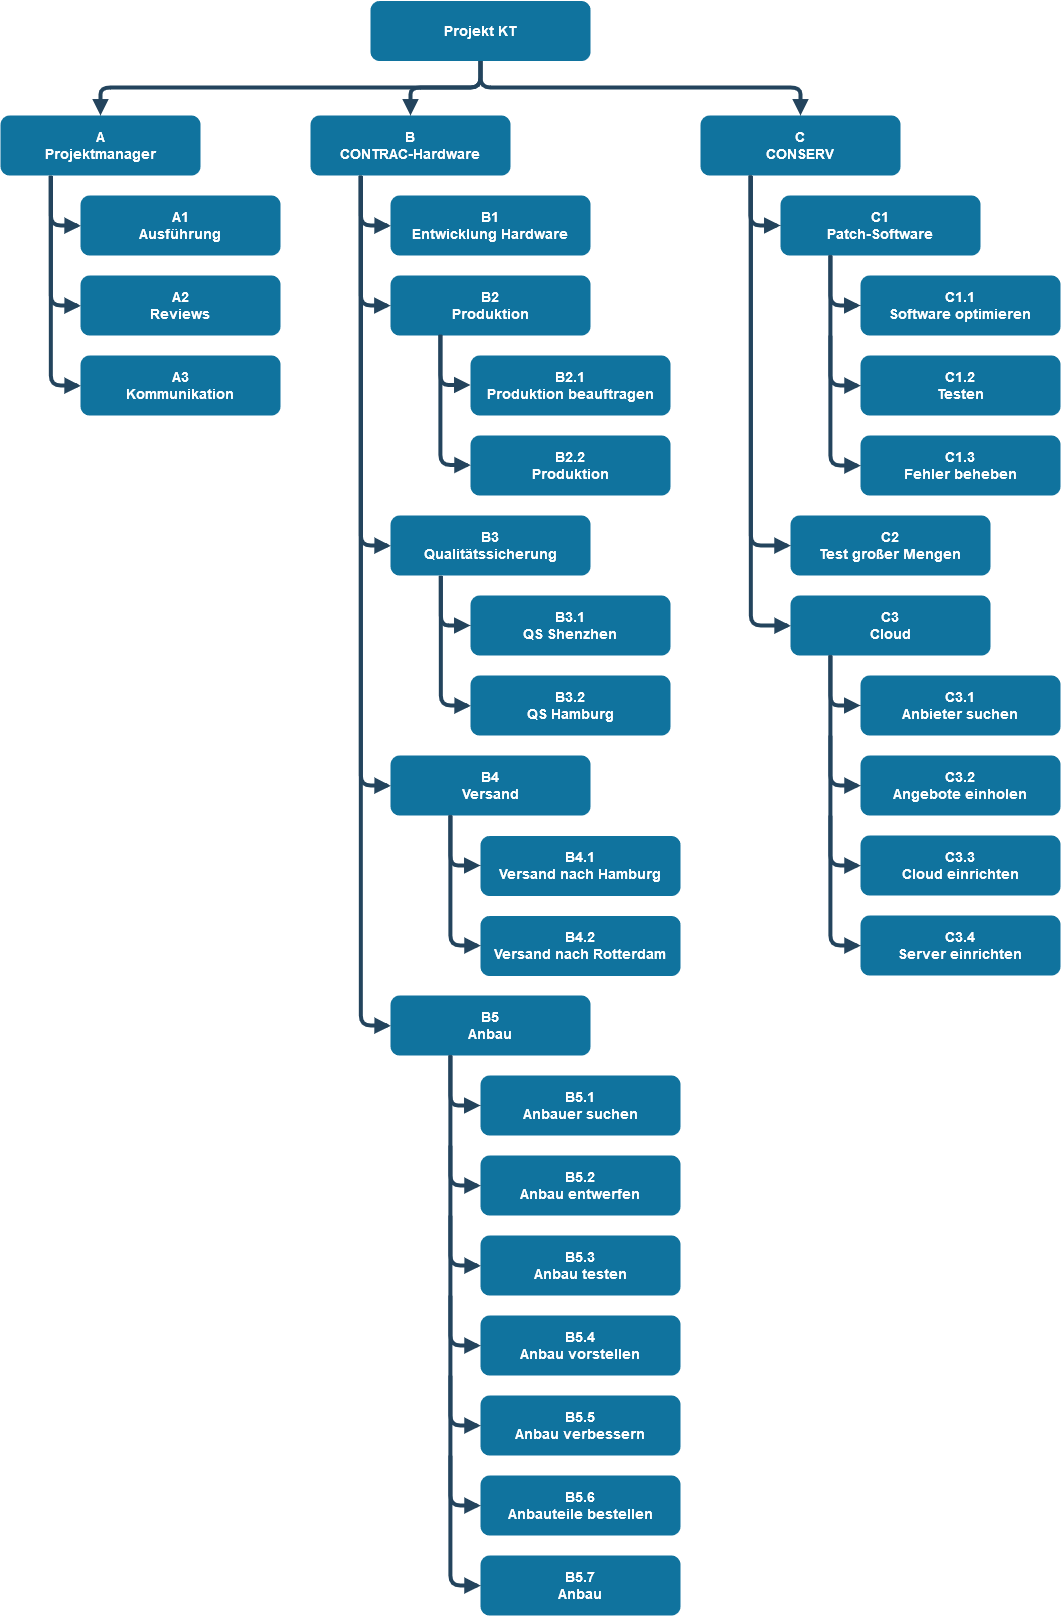
\includegraphics[width=0.8\textwidth]{WBS.png}
    \end{center}
    \caption{Work-Breakdown-Strukture}
\end{figure}
\subsection{Oranisation Breakdown Strukture}
\begin{figure}[H]
    \begin{center}
        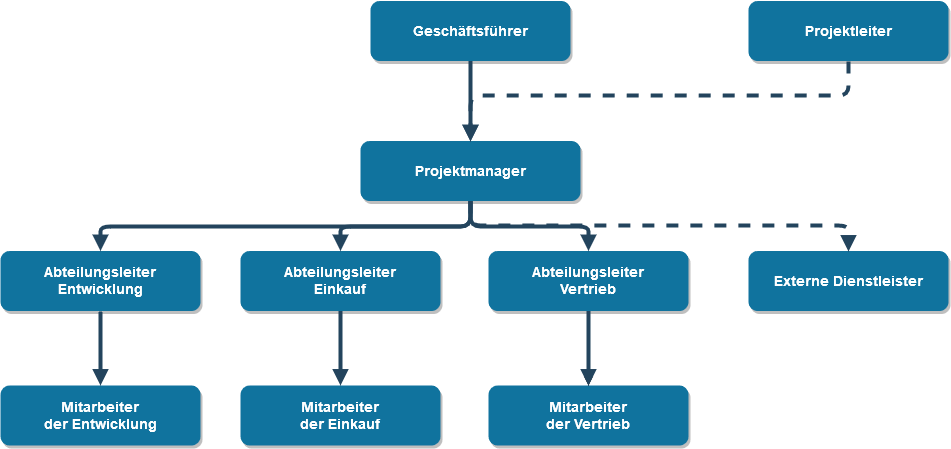
\includegraphics[width=0.8\textwidth]{OBS.png}
    \end{center}
    \caption{Organisation-Breakdown-Strukture}
\end{figure}
\section{Zeitmanagement}
\subsection{Aktivitätendauer}
\begin{table}[H]
    \renewcommand{\arraystretch}{1.1}
    \begin{center}
        \begin{tabular}{l|l|l}
            \hline
                        \textbf{ID} & \textbf{Aktivität} & \textbf{Dauer in d}\\\hline
            A    & \multicolumn{2}{l}{Projektmanager}\\ \hline
            A1   & Ausführungen                                        &120\\\hline
            A2   & Reviews                                             &22\\ \hline
            A3	 & Kommunikation									&120\\ \hline
            B    & \multicolumn{2}{l}{CONTRAC}\\ \hline
            B1   & Entwicklung Hardware &\\ \hline
            B2.1 & Produktion beauftragen                              &1\\ \hline
            B2.2 & Produktion                                          &30\\ \hline
            B3.1 & QS Shenzhen                                         &8\\ \hline
            B4.1 & Versand                                             &30\\ \hline
            B3.2 & QS Hamburg                                          &8\\ \hline
            B4.2 & Versand Rotterdam                                   &7\\ \hline
            B5.1 & Anbauer Suchen                                      &2\\ \hline
            B5.2 & Anbau entwerfen                                     &5\\ \hline
            B5.3 & Anbau testen                                        &2\\ \hline
            B5.4 & Anbau vorstellen                                    &2\\ \hline
            B5.5 & Anbau verbessern                                    &5\\ \hline
            B5.6 & Anbauteile bestellen                                &1\\ \hline
            B5.7 & Anbau                                               &3\\ \hline
            C    & \multicolumn{2}{l}{CONSERV}\\ \hline
            C1.1 & Patch-Software optimieren                           &30\\ \hline
            C1.2 & Patch-Software testen                               &20\\ \hline
            C1.3 & Patch-Software Fehler beheben                       &20\\ \hline
            C2   & Mit 5500 Geräten testen                             &10\\ \hline
            C3.1 & Cloud-Anbieter suchen                               &5\\ \hline
            C3.2 & Angebote einholen                                   &10\\ \hline
            C3.3 & Cloud einrichten                                    &10\\ \hline
            C3.4 & Server einrichten                                   &10\\ \hline
            D    & \multicolumn{2}{l}{CONTRAC-Firmware}\\ \hline
            D1   & ZigBee einbauen                                     &10\\ \hline
            D2.1 & Patch-Funktion optimieren                           &20\\ \hline
            D2.2 & Patch-Funktion testen                               &20\\ \hline
            D2.3 & Patch-Funktion Fehler beheben                       &10\\
        \end{tabular}
        \caption{Dauer der Aktivitäten im Projekt}
    \end{center}
\end{table}

\subsection{Meilensteine}

\subsection{PERT} % Kritischer Pfad !

\subsection{Gant} % Kritischer Pfad !

\section{Kommunikationsplan}
\subsection{Stakeholder}
\begin{table}[H]
    \renewcommand{\arraystretch}{1.1}
    \begin{center}
        \begin{tabular}{l|l}
            \textbf{Stakeholder} & \textbf{Kürzel}\\\hline
            
            
            
            
        \end{tabular}
    \end{center}
    \caption{Stakeholder}
\end{table}
\subsection{Regelmeetings} % Wer, wo, wann, wie oft, Medien?


\subsubsection{Dayly}


\subsubsection{Weekly Review}


\subsection{Statusberichte} % Wo gesammelt und verteilt


\subsubsection{Template für Statusberichte}



\section{Qualität}
\subsection{Qualitätsprozesse}
Um die Qualität der Hardware und Software werden bei EZ verschieden Prozesse eingesetzt. Dazu gehört eine doppelte Qualitätskontrolle der Hardware, Code Reviews sowie ausführliche und automatisierte Tests für die Software.
\subsection{Qualitätskontrolle der Hardware}
Alle CONTRAC-Geräte werden in Shenzhen und in Hamburg durch eine elektrische Kontrolle auf ihre Funktionalität geprüft.
\subsubsection{Code Review}
Jeder Code muss vor dem Mergen in den master-Branch durch einen zweiten Entwickler getestet und kontrolliert werden.
\subsubsection{Unit Test}
Für jede Softwarekomponente muss ein Unit-Test erstellt werden, der vor jedem Einchecken erfolgreich durchgeführt werden muss. Auch der Build-Server des Continuous-Integration-Zyklus muss die Tests erfolgreich ausführen. Bei einem Fehlschlag muss dieser zeitnah behoben werden.
\subsubsection{Test}
Jede erstellte Komponente muss vom Entwickler ausführlich getestet werden. Jede Komponente muss auch von einem zweiten Mitarbeiter getestet werden.
\subsection{Ticketsytem}
Als Ticktsystem kommt das firmeneigene Jira zum Einsatz. Dieses ist über die Adresse \texttt{https://jira.ez.de} verfügbar. Alle Entwickler und Product Owner besitzen ein Zugang zu diesem System.
\subsection{Versionierungssystem}
Als Versionierungssystem für das Projekt wird Git eingesetzt. Dieses ist allen Entwicklern auf ihren Computern verfügbar. Als Git-Remote dient der firmeneigene Bitbucket-Server, der unter der Adresse \texttt{git.ez.de} verfügbar ist. Auch aus dem Internet ist der Server unter dieser Adresse verfügbar.

Eine Commit-Message muss immer die getätigte Arbeit beschreiben und eine eindeutige Zuordung zu einem Ticket oder ein User Story ermöglichen. Dazu werden diese über ihre eindeutige Bezeichnung (US-3, BUG-5) erwähnt.
\subsection{Codestyle}
Der geschriebene Code muss den Stylerichtlinien der Firma entsprechen. Diese können dem hausinternen Wiki unter \texttt{wiki.ez.de} entnommen werden. Konfigurationsdateien für verschiedene IDEs und Formatierer können dort auch heruntergeladen werden. Diese Richtlinien werden auch an externe Firmen weitergegeben. 
\subsection{Bugverlauf}
Jeder entdeckte Bug muss in Jira dokumentiert werden. Die Bugs fließen dann in die Backlogs für die Entwicklung ein. Dort werden sie mit erhöhter Priorität belegt.
\section{Risikoplan}
\subsection{Annahmen} % Auswahl



\subsection{Risiken mit Priorität} %3 Stück


\subsection{Bewertung } %Wahrscheinlichkeitsanalyse, Risikomatrix


\subsection{Risikokosten}


\section{Human Ressources}
\subsection{Aufgabenverteilung}
\begin{table}[H]
    \renewcommand{\arraystretch}{1.1}
    \begin{center}
        \begin{tabular}{l|l}
            \hline
            A    & Projektmanager                                      \\ \hline
            A1   & Ausführungen                                        \\ \hline
            A2   & Reviews                                             \\ \hline
                        A3 & Kommunikation \\\hline
            &                                                     \\ \hline
            B    & CONTRAC                                             \\ \hline
            B1   & Entwicklung Verbesserung Hardware (ZigBee und Akku) \\ \hline
            B2.1 & Produktion beauftragen                              \\ \hline
            B2.2 & Produktion                                          \\ \hline
            B3.1 & QS Shenzhen                                         \\ \hline
            B4.1 & Versand                                             \\ \hline
            B3.2 & QS Hamburg                                          \\ \hline
            B4.2 & Versand Rotterdam                                   \\ \hline
            B5.1 & Anbauer Suchen                                      \\ \hline
            B5.2 & Anbau entwerfen                                     \\ \hline
            B5.3 & Anbau testen                                        \\ \hline
            B5.4 & Anbau vorstellen                                    \\ \hline
            B5.5 & Anbau verbessern                                    \\ \hline
            B5.6 & Anbauteile bestellen                                \\ \hline
            B5.7 & Anbau                                               \\ \hline
            &                                                     \\ \hline
            C    & CONSERV                                             \\ \hline
            C1.1 & Patch-Software optimieren                           \\ \hline
            C1.2 & Patch-Software testen                               \\ \hline
            C1.3 & Patch-Software Fehler beheben                       \\ \hline
            C2   & Mit 5500 Geräten testen                             \\ \hline
            C3.1 & Cloud-Anbieter suchen                               \\ \hline
            C3.2 & Angebote einholen                                   \\ \hline
            C3.3 & Cloud einrichten                                    \\ \hline
            C3.4 & Server einrichten                                   \\ \hline
            &                                                     \\ \hline
            D    & CONTRAC-Firmware                                    \\ \hline
            D1   & ZigBee einbauen                                     \\ \hline
            D2.1 & Patch-Funktion optimieren                           \\ \hline
            D2.2 & Patch-Funktion testen                               \\ \hline
            D2.3 & Patch-Funktion Fehler beheben                       \\
        \end{tabular}
        \caption{Aufgabenverteilung im Projekt}
    \end{center}
\end{table}
\subsection{Aktionsplan}



\subsection{Motivation} % Teamevents, Awards .. (kostet Geld)



\section{Beschaffung} % UserStories an extenern Firma
Bei der Firma DOTDAT GmbH wird die Entwicklung der Hardware eingekauft. Die von DOTDAT angefragten UserStories lauten wie folgt:



\section{Kostenmanagement}



\subsection{Kostenschätzung}
\lipsum[2]
\subsection{Personalkosten} % Awards, Reise, Hotel, Betriebssätze ...
\lipsum[2]
\subsection{Materialkosten}
\lipsum[2]
\subsection{Risikokosten}
\lipsum[2]
\subsection{Gewinnmarge}
\lipsum[2]
\subsection{Kontigenz} %
\lipsum[2]
\subsection{Plankosten}
\lipsum[2]









% Verzeichnisse
\clearpage
\listoffigures
%\cleardoublepage

\listoftables
%\cleardoublepage

%\lstlistoflistings
%\cleardoublepage

%\newcommand{\abkvz}{Abkürzungsverzeichnis}
%\renewcommand{\nomname}{\abkvz}
%\section*{\abkvz}
%\markboth{\abkvz}{\abkvz}
%\addcontentsline{toc}{section}{\abkvz}
%% !TEX root = Ausarbeitung.tex

% Es werden nur die Abkürzungen aufgelistet, die mit \ac definiert und auch benutzt wurden. 
%
% \acro{VERSIS}{Versicherungsinformationssystem\acroextra{ (Bestandsführungssystem)}}
% Ergibt in der Liste: VERSIS Versicherungsinformationssystem (Bestandsführungssystem)
% Im Text aber: \ac{VERSIS} -> Versicherungsinformationssystem (VERSIS)

% Hinweis: allgemein bekannte Abkürzungen wie z.B. bzw. u.a. müssen nicht ins Abkürzungsverzeichnis aufgenommen werden
% Hinweis: allgemein bekannte IT-Begriffe wie Datenbank oder Programmiersprache müssen nicht erläutert werden,
%          aber ggfs. Fachbegriffe aus der Domäne des Prüflings (z.B. Versicherung)

% Die Option (in den eckigen Klammern) enthält das längste Label oder
% einen Platzhalter der die Breite der linken Spalte bestimmt.
\begin{acronym}[WWWWW]
	\acro{API}{Application Programming Interface}
	\acro{CI}{Continous Integration}
	\acro{IDE}{Integrated Development Environment}
	\acro{SDK}{Software Development Kit}
	\acro{SaSS}{Software as a Service}
    \acro{UI}{Benutzeroberfläche (engl.: "`User Interface"')}
    \acro{VCS}{Version Control System}
    \acro{CI}{Kontinuierliche Integration (engl.: "Continuous Integration")}
    \acro{VM}{Virtuelle Maschine}
    \acro{CPU}{Central Processing Unit}
    \acro{SPARC}{Scalable Processor ARChitecture}
    \acro{LXC}{Linux Containers}
    \acro{OCI}{Open Container Initiative}
\end{acronym}


% Literatur ------------------------------------------------------------------

%\renewcommand{\refname}{Literaturverzeichnis}
%\bibliography{Bibliographie}
%\bibliographystyle{Allgemein/natdin} % DIN-Stil des Literaturverzeichnisses
%\bibliographystyle{alphadin}
%% !TEX root = Projektdokumentation.tex
\clearpage
\addsec{Eidesstattliche Erklärung}

% Hinweis: die eidesstattliche Erklärung ist ggfs. an die Richtlinie der IHK anzupassen

Ich, \autorName, versichere hiermit, dass ich meine \textbf{\betreff} mit dem
Thema
\begin{quote}
\textit{\kompletterTitel}
\end{quote}
selbständig verfasst und keine anderen als die angegebenen Quellen und Hilfsmittel benutzt habe,
wobei ich alle wörtlichen und sinngemäßen Zitate als solche gekennzeichnet habe. Die Arbeit
wurde bisher keiner anderen Prüfungsbehörde vorgelegt und auch nicht veröffentlicht.\\[6ex]

\abgabeOrt, den \abgabeTermin


\rule[-0.2cm]{5.5cm}{0.5pt}

\textsc{\autorName}
 % Eidesstattliche Erklärung nur wenn von nöten drucken

% Anhang ---------------------------------------------------------------------
\clearpage
\appendix
\pagenumbering{Roman}
% !TEX root = Ausarbeitung.tex
\section{Anhang}
\label{sec:anhang}





\end{document}
